% !TeX spellcheck = en_US
%!TEX options = -shell-escape
\documentclass[12pt,fleqn,twoside,a4paper]{article}
\usepackage{etex}
% Select encoding of your inputs.
\usepackage[utf8]{inputenc}

% Make latex understand and use the typographic
% rules of the language used in the document.
\usepackage[english, danish]{babel}

% Use the vector font Latin Modern which is going
% to be the default font in latex in the future.
\usepackage{lmodern}
% Use vector arrows in mathmode
\usepackage{esvect}

% Choose the font encoding
\usepackage[T1]{fontenc}

% load a colour package
\usepackage[table]{xcolor}
\definecolor{aaublue}{RGB}{33,26,82}% dark blue

% The standard graphics inclusion package
\definecolor{white}{RGB}{255,255,255} % define color white
\usepackage{graphicx}

% Set up how figure and table captions are displayed
\usepackage{caption}
\captionsetup{%
  font=footnotesize,% set font size to footnotesize
  labelfont=bf % bold label (e.g., Figure 3.2) font
}

% Enable row combination in tables
\usepackage{multirow}

% Make space between table lines and text
\renewcommand{\arraystretch}{1.5}

% Make the standard latex tables look so much better
\usepackage{array,booktabs}

% Enable the use of frames around, e.g., theorems
% The framed package is used in the example environment
\usepackage{framed}
\usepackage{colortbl}
\usepackage{longtable}

\usepackage{textcomp}

%%%%%%%%%%%%%%%%%%%%%%%%%%%%%%%%%%%%%%%%%%%%%%%%
% Mathematics
%%%%%%%%%%%%%%%%%%%%%%%%%%%%%%%%%%%%%%%%%%%%%%%%
% Defines new environments such as equation,
% align and split 
\usepackage{mathrsfs,amsmath}
\usepackage{relsize}
% Adds new math symbols
\usepackage{amssymb}
% Use theorems in your document
% The ntheorem package is also used for the example environment
% When using thmmarks, amsmath must be an option as well. Otherwise \eqref doesn't work anymore.
\usepackage[framed,amsmath,thmmarks]{ntheorem}

%%%%%%%%%%%%%%%%%%%%%%%%%%%%%%%%%%%%%%%%%%%%%%%%
% Page Layout
%%%%%%%%%%%%%%%%%%%%%%%%%%%%%%%%%%%%%%%%%%%%%%%%
% Change margins, papersize, etc of the document
\usepackage[
  left=25mm,% left margin on an odd page %tidligere 25mm for baade right og left
  right=25mm,% right margin on an odd page
  top=35mm,
  ]{geometry}
  
% Modify how \chapter, \section, etc. look
% The titlesec package is very configureable
\usepackage{titlesec}
\makeatletter
\def\ttl@mkchap@i#1#2#3#4#5#6#7{%
    \ttl@assign\@tempskipa#3\relax\beforetitleunit
    \vspace{\@tempskipa}%<<<<<< REMOVE THE * AFTER \vspace
    \global\@afterindenttrue
    \ifcase#5 \global\@afterindentfalse\fi
    \ttl@assign\@tempskipb#4\relax\aftertitleunit
    \ttl@topmode{\@tempskipb}{%
        \ttl@select{#6}{#1}{#2}{#7}}%
    \ttl@finmarks  % Outside the box!
    \@ifundefined{ttlp@#6}{}{\ttlp@write{#6}}}
\makeatother

\titlespacing{\chapter}{0pt}{0pt}{10pt}
\titlespacing{\section}{0pt}{0pt}{-5pt}
\titlespacing{\subsection}{0pt}{8pt}{-5pt}
\titlespacing{\subsubsection}{0pt}{6pt}{-10pt}

%\titleformat*{\section}{\normalfont\Large\bfseries}\color{aaublue}}
\titleformat{\section}
  {\normalfont\scshape}{\thesection}{1em}{}

\titleformat*{\subsection}{\normalfont\large\bfseries}%\color{aaublue}}
\titleformat*{\subsubsection}{\normalfont\normalsize\bfseries}%\color{aaublue}}
%\titleformat*{\paragraph}{\normalfont\normalsize\bfseries\color{aaublue}}
%\titleformat*{\subparagraph}{\normalfont\normalsize\bfseries\color{aaublue}}

%Formatting chapter headers. Predefined styles that can be used as option to the package: Sonny, Lenny, Glenn, Conny, Rejne, Bjarne, PetersLenny and Bjornstrup

%\usepackage[Sonny]{fncychap}

\usepackage{titlesec, blindtext, color}
%\definecolor{gray75}{gray}{0.75}
\newcommand{\hsp}{\hspace{20pt}}
%\titleformat{\chapter}[hang]{\Huge\bfseries}{\thechapter\hsp{|}\hsp}{0pt}{\Huge\bfseries}
\titleformat{\chapter}[hang]{\bfseries}{\thechapter\hsp{|}\hsp}{0pt}{\bfseries}


% Change the headers and footers
\usepackage{fancyhdr}
\setlength{\headheight}{15pt}
\pagestyle{fancy}
\fancyhf{} %delete everything
\renewcommand{\headrulewidth}{0pt} %remove the horizontal line in the header
\fancyhead[RO,LE]{\small\nouppercase\leftmark} %even page - chapter title

\fancyhead[LO]{}
\fancyhead[RE]{} 
\fancyhead[CE]{}
\fancyhead[CO]{}

\fancyfoot[RE,LO]{\thepage}
\fancyfoot[LE,RO]{B205} %page number on all pages
\fancyfoot[CE,CO]{}



% change first page of all chapters header and footer to fancy style
\makeatletter
\let\ps@plain\ps@fancy
\makeatother

% Do not stretch the content of a page. Instead,
% insert white space at the bottom of the page
\raggedbottom

% Enable arithmetics with length. Useful when typesetting the layout.
\usepackage{calc}

%%%%%%%%%%%%%%%%%%%%%%%%%%%%%%%%%%%%%%%%%%%%%%%%
% Bibliography
%%%%%%%%%%%%%%%%%%%%%%%%%%%%%%%%%%%%%%%%%%%%%%%%
% Add the \citep{key} command which display a
% reference as [author, year]
\usepackage[square]{natbib}
\usepackage{natbib}
% Appearance of the bibliography
\bibliographystyle{00setup/apalike}
%\bibliographystyle{IEEEtran}

%%%%%%%%%%%%%%%%%%%%%%%%%%%%%%%%%%%%%%%%%%%%%%%%
% Misc
%%%%%%%%%%%%%%%%%%%%%%%%%%%%%%%%%%%%%%%%%%%%%%%%

% Add bibliography and index to the table of
% contents
\usepackage[nottoc, notlof, notlot]{tocbibind}
\usepackage{tocloft}
% Add the command \pageref{LastPage} which refers to the
% page number of the last page
\setlength{\cftbeforetoctitleskip}{0 cm}

\usepackage[
  %disable, %turn off todonotes
  colorinlistoftodos, %enable a coloured square in the list of todos
  %inline,
  textwidth=20mm, %set the width of the todonotes
  textsize=scriptsize, %size of the text in the todonotes
  ]{todonotes}
\setlength{\marginparwidth}{2cm}
\newcommand{\todocheck}[1]{\todo[color=green!40, author=Check]{#1}}
\newcommand{\todojens}[1]{\todo[color=red!40, author=Jens, inline]{#1}}
%Command for inserting green todo notes as Ole's corrections.
%\renewcommand{\todo}[1]{\todo[noline]{#1}}  
    
\usepackage{wrapfig}
\usepackage{amssymb}
\usepackage{pifont}
% Enables figures with text wrapped tightly around it 

%%% Table of contents %%%%%  
\setcounter{tocdepth}{1}

\renewcommand{\cftpartpresnum}{Part~}
\let\cftoldpartfont\cftpartfont
\renewcommand{\cftpartfont}{\cftoldpartfont\cftpartpresnum}

%%%%%%%%%%%%%%%%%%%%%%%%%%%%%%%%%%%%%%%%%%%%%%%%
% Hyperlinks
%%%%%%%%%%%%%%%%%%%%%%%%%%%%%%%%%%%%%%%%%%%%%%%%

% Enable hyperlinks and insert info into the pdf
% file. Hypperref should be loaded as one of the 
% last packages
\usepackage{nameref}
\usepackage{hyperref}
\hypersetup{%
	%pdfpagelabels=true,%
	plainpages=false,%
	pdfauthor={Author(s)},%
	pdftitle={Title},%
	pdfsubject={Subject},%
	bookmarksnumbered=true,%
	colorlinks,%
	citecolor=black,%
	filecolor=black,%
	linkcolor=black,% you should probably change this to black before printing
	urlcolor=black,%
	pdfstartview=FitH%
}

% remove all indentations
\setlength\parindent{0pt}
\parskip 5mm
\usepackage{verbatim}


\definecolor{Gra}{RGB}{230,230,230}

%creates a nice-looking C#-text
\newcommand{\CC}{C\nolinebreak\hspace{-.05em}\raisebox{.3ex}{\scriptsize\text \#} }

%enables multi column lists
\usepackage{multicol}

%enables code-examples
\usepackage{listings}

\definecolor{coolblue}{RGB}{32,95,128}
\definecolor{mygreen}{rgb}{0,0.6,0}
\definecolor{mygray}{rgb}{0.5,0.5,0.5}
\definecolor{mymauve}{rgb}{0.58,0,0.82}
\usepackage{textcomp}
\definecolor{listinggray}{gray}{0.9}
\definecolor{lbcolor}{rgb}{0.9,0.9,0.9}


%%%%%%%%%%%%%%%%%%%%%%%%%%%%%%%%%%%%%%%%%%%%%%%%
% Listing
%%%%%%%%%%%%%%%%%%%%%%%%%%%%%%%%%%%%%%%%%%%%%%%%

\usepackage{xcolor}
\colorlet{keyword}{blue!90!black!100}
\colorlet{keyword2}{red!40!blue!85}
\colorlet{comment}{green!60!black!100}
\definecolor{backcolour}{rgb}{0,0,0}
\usepackage{beramono}% monospaced font with bold variant
\definecolor{backcolourlst}{rgb}{0.97,0.97,0.96}
%\definecolor{backcolourlst}{rgb}{1,0.75,0.80}

\lstset{
%  backgroundcolor=\color{white},   % choose the background color; you must add \usepackage{color} or \usepackage{xcolor}
%  basicstyle=\footnotesize,        % the size of the fonts that are used for the code
%  breakatwhitespace=false,         % sets if automatic breaks should only happen at whitespace
%  breaklines=true,                 % sets automatic line breaking
%  captionpos=t,                    % sets the caption-position to bottom
%  commentstyle=\color{mygreen},    % comment style
%  deletekeywords={...},            % if you want to delete keywords from the given language
%  escapeinside={\%*}{*)},          % if you want to add LaTeX within your code
%  extendedchars=true,              % lets you use non-ASCII characters; for 8-bits encodings only, does not work with UTF-8
%  frame=single,                    % adds a frame around the code
%  keepspaces=true,                 % keeps spaces in text, useful for keeping indentation of code (possibly needs columns=flexible)
%  keywordstyle=\color{blue},       % keyword style
%  language=C++,                 % the language of the code
%  morekeywords={*,...},            % if you want to add more keywords to the set
%  numbers=left,                    % where to put the line-numbers; possible values are (none, left, right)
%  numbersep=5pt,                   % how far the line-numbers are from the code
%  numberstyle=\tiny\color{mygray}, % the style that is used for the line-numbers
%  rulecolor=\color{black},         % if not set, the frame-color may be changed on line-breaks within not-black text (e.g. comments (green here))
%  showspaces=false,                % show spaces everywhere adding particular underscores; it overrides 'showstringspaces'
%  showstringspaces=false,          % underline spaces within strings only
%  showtabs=false,                  % show tabs within strings adding particular underscores
%  stepnumber=1,                    % the step between two line-numbers. If it's 1, each line will be numbered
%  stringstyle=\color{mymauve},     % string literal style
%  tabsize=2,                       % sets default tabsize to 2 spaces
%  title=\lstname                   % show the filename of files included with \lstinputlisting; also try caption instead of title
	backgroundcolor=\color{lbcolor},
	tabsize=4,
	rulecolor=\color{black},
	language=C,
  	basicstyle   = \linespread{1.2} \ttfamily \scriptsize,
  	keywordstyle = \color{keyword}\bfseries,	
  	commentstyle = \color{comment}\bfseries,
  	numbers=left,                   
	numberstyle=\scriptsize,      
	stepnumber=1,                   
	numbersep=8pt,                  
	backgroundcolor=\color{white},  
	showspaces=false,               
	showstringspaces=false,         
	showtabs=false,                 
	backgroundcolor=\color{backcolourlst},
	%frame=single,
	frame=single,                   
	captionpos=b,           
	breaklines=true,        
	breakatwhitespace=false,    
	escapeinside={\%*}{*)}
}
\lstset{
	emph={uint8, int8_t, uint16_t, int16, uint32_t, int32_t,}, emphstyle={\color{keyword}\bfseries},
    emph={[2]ISR, TCE1, CNT, TCC1, TCD1_OVF_vect},emphstyle={[2]\color{keyword2}\bfseries}%
}



\usepackage{float}
\usepackage{caption}
\usepackage{subcaption}
\usepackage{siunitx}
\sisetup{decimalsymbol=comma}
\sisetup{detect-weight}

\usepackage{enumitem}
%\usepackage[citestyle=authoryear,natbib=true]{biblatex}

% Figures - TIKZ
\usepackage{tikz}
\usepackage[americanresistors,americaninductors,americancurrents, americanvoltages]{circuitikz}


% Wall of text logo

\newcommand{\walloftextalert}[0]{\includegraphics[width=\textwidth]{walloftext.png}}


% Citation aliasses for nicer references in text
\defcitealias{ISO226}{\scshape ISO223, 2003}
\defcitealias{radio_standard}{\scshape IEC 61305-2, 1997}
\defcitealias{tysk}{\scshape EN 60315-4, 1998}
\defcitealias{REC}{\scshape Rec. ITU-R BS.704, 1990}
\defcitealias{std581}{\scshape IEC 581-6, 1979}
\defcitealias{std1305}{\scshape IEC 1305-3, 1995}
\defcitealias{std268-3}{\scshape IEC 60268-3, 2000}
\defcitealias{DS61938}{\scshape DS/EN 61938, 1997}
\defcitealias{std581-8}{\scshape IEC 581-8, 1987}


% URL break fix nede i bibfil

\def\UrlBreaks{\do\/\do-}


\usepackage{pdfpages}

\definecolor{blockcolor}{RGB}{112,168,218}

\tikzstyle{blockbig} = [draw, fill=blockcolor, rectangle, 
    minimum height=3em, minimum width=6em]
\tikzstyle{block} = [draw, fill=blockcolor, rectangle, 
    minimum height=2em, minimum width=2em]
    
\tikzstyle{blockbigclear} = [draw, fill=white, rectangle, 
    minimum height=3em, minimum width=6em]
\tikzstyle{blockclear} = [draw, fill=white, rectangle, 
    minimum height=2em, minimum width=2em]
    
\tikzstyle{sum} = [draw, fill=blockcolor, circle, node distance=1.5cm, minimum size=0.6cm]
\tikzstyle{sumclear} = [draw, fill=white, circle, node distance=1.5cm, minimum size=0.6cm]
\tikzstyle{input} = [coordinate]
\tikzstyle{output} = [coordinate]
\tikzstyle{pinstyle} = [pin edge={to-,thin,black}]

%% Centering columns of custom width
\newcolumntype{P}[1]{>{\centering\arraybackslash}p{#1}}
\newcolumntype{M}[1]{>{\centering\arraybackslash}m{#1}}

\usepackage{empheq}
\newcommand*\widefbox[1]{\fbox{\hspace{2em}#1\hspace{2em}}}

\newcommand{\todoanders}[1]{\todo[color=red!40, author=Anders]{#1}}
\graphicspath{{./rapport/billeder/}}
\newcommand{\todohusk}[1]{\todo[color=red, author=HUSK:]{#1}}


\makeatletter
\renewcommand{\todo}[2][]{\tikzexternaldisable\@todo[#1]{#2}\tikzexternalenable}
\renewcommand{\missingfigure}[2][]{\tikzexternaldisable\@missingfigure[#1]{#2}\tikzexternalenable}
\makeatother


%%PGF TABLES%%
\usepackage{booktabs}
\newcommand{\ra}[1]{\renewcommand{\arraystretch}{#1}}
\usepackage{array}
\usepackage{ragged2e}

\newcommand*{\textlabel}[2]{				% Gør \textlabel mulig
  \edef\@currentlabel{#1}					% Set target label
  \phantomsection							% Correct hyper reference link
  #1\label{#2}}								% Print and store label

% ¤¤ Opsætning af enheder ¤¤ % 
\newcommand{\enhed}[1]{\hfill[\mathrm{#1}]}   % Skriv \enhed{"din enhed"} og dem bliver rykket til højre



\usepackage{multicol}
\usepackage{lipsum}
\usepackage{lettrine}% package inclusion and set up of the document
%Creates the aau titlepage
\newcommand{\aautitlepage}[3]{%
  {
    %set up various length
    \ifx\titlepageleftcolumnwidth\undefined
      \newlength{\titlepageleftcolumnwidth}
      \newlength{\titlepagerightcolumnwidth}
    \fi
    \setlength{\titlepageleftcolumnwidth}{0.5\textwidth-\tabcolsep}
    \setlength{\titlepagerightcolumnwidth}{\textwidth-2\tabcolsep-\titlepageleftcolumnwidth}
    %create title page
    \thispagestyle{empty}
    \noindent%
    \begin{tabular}{@{}ll@{}}
      \parbox{\titlepageleftcolumnwidth}{
        \iflanguage{danish}{%
          \includegraphics[width=\titlepageleftcolumnwidth]{00setup/aau_logo_da.pdf}
        }{%
          \includegraphics[width=\titlepageleftcolumnwidth]{00setup/aau_logo_en.pdf}
        }
      } &
      \parbox{\titlepagerightcolumnwidth}{\raggedleft\sf\small
        #2
      }\bigskip\\
       #1 &
      \parbox[t]{\titlepagerightcolumnwidth}{%
      \textbf{Abstract:}\smallskip\par
        \fbox{\parbox{\titlepagerightcolumnwidth-2\fboxsep-2\fboxrule}{%
          #3
        }}
      }\\
    \end{tabular}
    \vfill
    \vspace{-0.5cm}
    \iflanguage{danish}{%
      \noindent{\footnotesize\emph{Rapportens indhold er frit tilgængeligt, men offentliggørelse (med kildeangivelse) må kun ske efter aftale med forfatterne.}}
    }{%
      \noindent{\footnotesize\emph{The content of this report is freely available, but publication (with reference) may only be pursued due to agreement with the author.}}
    }
    \clearpage
  }
}

%Create english project info
\newcommand{\englishprojectinfo}[8]{%
  \parbox[t]{\titlepageleftcolumnwidth}{
    \textbf{Title:}\\ #1\bigskip\par
    \textbf{Theme:}\\ #2\bigskip\par
    \textbf{Project Period:}\\ #3\bigskip\par
    \textbf{Project Group:}\\ #4\bigskip\par
    \textbf{Participant(s):}\\ #5\bigskip\par
    \textbf{Supervisor(s):}\\ #6\bigskip\par
    \textbf{Copies:} #7\bigskip\par
    \textbf{Page Numbers:} Fucking mange!\bigskip\par
    \textbf{Date of Completion:}\\ #8
  }
}

%Create danish project info
\newcommand{\danishprojectinfo}[9]{%
  \parbox[t]{\titlepageleftcolumnwidth}{
    \textbf{Title:}\\ #1\bigskip\par
    \textbf{Theme:}\\ #2\bigskip\par
    \textbf{Project Period:}\\ #3\bigskip\par
    \textbf{Project Group:}\\ #4\bigskip\par
    \textbf{Participants:}\\ #5\bigskip\par
    \textbf{Supervisor:}\\ #6\bigskip\par
    \textbf{}\\ #7\bigskip\par
    \textbf{Page Numbers:} 119\bigskip\par
    \textbf{Date of Completion:}\\ #9
  }
}

%Nice-looking reference to other chapters
\newcommand{\chapref}[1]{Chapter \ref{#1}: \nameref{#1}}
\newcommand{\secref}[1]{Section \ref{#1}: \nameref{#1}}
\newcommand{\figref}[1]{figure \ref{#1}}
\newcommand{\appref}[1]{Appendix \ref{#1}}
\newcommand{\tabref}[1]{\emph{Table: \ref{#1}}}
\newcommand{\coderef}[1]{\emph{Listings: \ref{#1}}}
\renewcommand{\eqref}[1]{eq. (\ref{#1})}

\renewcommand{\equationautorefname}{eq. }
\renewcommand{\figureautorefname}{figure }

\newcommand{\iic}[0]{I²C }

%%%%%%%%%%%%%%%%%%%%%%%%%%%%%%%%%%%%%%%%%%%%%%%%
% An example environment
%%%%%%%%%%%%%%%%%%%%%%%%%%%%%%%%%%%%%%%%%%%%%%%%
\theoremheaderfont{\normalfont\bfseries}
\theorembodyfont{\normalfont}
\theoremstyle{break}
\def\theoremframecommand{{\color{aaublue!50}\vrule width 5pt \hspace{5pt}}}
%\newshadedtheorem{exa}{Example}[chapter]
\newenvironment{example}[1]{%
		\begin{exa}[#1]
}{%
		\end{exa}
}

\makeatletter
\newcommand{\ChapterOutsidePart}{%
   \def\toclevel@chapter{-1}\def\toclevel@section{0}\def\toclevel@subsection{1}}
\newcommand{\ChapterInsidePart}{%
   \def\toclevel@chapter{0}\def\toclevel@section{1}\def\toclevel@subsection{2}}
\makeatother

\usepackage{bookmark}

\usepackage{mathtools}
\DeclarePairedDelimiter{\ceil}{\lceil}{\rceil}

%\newenvironment{where}{Where:\\}{\\}

\newcommand{\nomunit}[1]{\renewcommand{\nomentryend}{\hspace*{\fill}#1}}
% \usepackage{array} is required
% \usepackage{array} is required

\newcommand{\new}[3]{\begin{tabular}{p{10pt} p{40pt} p{230pt} l} 
&{#1} & {#2} & {$\left[\text{#3}\right]$}
\end{tabular} \vspace{3pt} \nomenclature{#1}{#2}{#3}{}}

\newcommand{\newpar}{\par \vspace{0.4cm}}



\newenvironment{where}{\hspace{6mm}Where:\\}{}
\newcommand{\va}[3]{\begin{tabular}{p{40pt} p{47pt} p{200pt} l} 
&{#1} & {#2} & {$\left[\text{#3}\right]$}
\end{tabular}}


% easy differential operators
\newcommand*\diff{\mathop{}\!\mathrm{d}}
\newcommand*\Diff[1]{\mathop{}\!\mathrm{d^#1}}
% my new macros
\input{00setup/glossaries.tex} % glossaries stuff
\usepackage{schemabloc}
\usetikzlibrary{shapes,arrows}
\usepackage{pgfplots}
\usetikzlibrary{plotmarks}
\pgfplotsset{compat=newest}
\pgfplotsset{filter discard warning=false}

\usetikzlibrary{external}
\tikzexternalize[prefix=tikz/]
\pgfdeclarelayer{bg}    % declare background layer
\pgfsetlayers{bg,main}


%\usepackage{silence}
%\WarningsOff[pgfplots]
%\WarningFilter{latex}{Marginpar on page}
%\WarningsOff[latex]


%%% Tikz Magic %%%
\tikzstyle{block} = [draw,rounded corners , rectangle, minimum height=3em, minimum width=6em]
\tikzstyle{Integrator} = [draw, fill=blue!20, rectangle, minimum height=5mm, minimum width=5mm]
\tikzstyle{Twolineblock} = [draw,rounded corners , rectangle, minimum height=3em, minimum width=6em, text width = 6em, align=center]     
\tikzstyle{sum} = [draw, fill=blue!20, circle, node distance=1cm]
\tikzstyle{input} = [coordinate]
\tikzstyle{output} = [coordinate]
\tikzstyle{pinstyle} = [pin edge={to-,thin,black}]
\tikzstyle{box} = [draw,rounded corners, minimum height=15mm, minimum width=20mm, align=center, text centered]
\tikzstyle{BlackBox} = [draw, fill=black, rounded corners, minimum height=15mm, minimum width=20mm, align=center, text=white, text centered]
\tikzstyle{FlowIF} = [diamond, draw, fill=blue!20, text width=8.5em, text badly centered, node distance=3cm, inner sep=0pt,align=center,aspect=3]
\tikzstyle{FlowBlock} = [rectangle, draw, fill=blue!20, text width=8em, text centered, rounded corners, minimum height=3em]
\tikzstyle{FlowCloud} = [draw, ellipse,fill=red!20, node distance=3cm, minimum height=2em]
\tikzstyle{TestBox} = [rectangle,draw, fill=black!20, minimum height=8mm, minimum width=8mm]
\tikzstyle{TestDiamond} = [diamond, draw, fill=black!20, minimum height=10.5mm, minimum width=10.5mm]
\tikzstyle{TestBox} = [rectangle,draw, fill=black!20, minimum height=8mm, minimum width=8mm]
\tikzstyle{TestCircle} = [circle, draw, fill=black!20, minimum height=6mm, minimum width=6mm]
\tikzstyle{TestTable} = [rectangle, draw, fill=black!60, minimum height=0.01mm, minimum width=9mm, text=white]
\tikzstyle{TestBoxSmall} = [rectangle,draw, fill=black!, minimum height=8mm, minimum width=8mm,text=white]
\tikzstyle{LegendBox} = [rectangle,draw, minimum height=7mm, minimum width=20mm]
\tikzstyle{Sysbox} = [draw,rounded corners, minimum height=15mm, minimum width=9em, align=center, text centered,text width = 10.5em]
\tikzstyle{SysBlackBox} = [draw, fill=black, text=white, rounded corners, minimum height=15mm, minimum width=9em, align=center, text centered,text width = 10em]
\tikzstyle{PreAmpBox} = [rectangle,draw, fill=black!20, minimum height=8mm, minimum width=12mm]
\tikzstyle{gain} = [fill=white, draw, rectangle, minimum height=2.5em, minimum width=2.5em]
\tikzstyle{summation} = [draw, minimum size=0.75cm, circle, node distance=1.75cm]












%% Its a pie chart!! %%%
\definecolor{rosso}{RGB}{220,57,18}
\definecolor{giallo}{RGB}{255,153,0}
\definecolor{blu}{RGB}{102,140,217}
\definecolor{verde}{RGB}{16,150,24}
\definecolor{viola}{RGB}{153,0,153}

\makeatletter

\tikzstyle{chart}=[
    legend label/.style={font={\scriptsize},anchor=west,align=left},
    legend box/.style={rectangle, draw, minimum size=5pt},
    axis/.style={black,semithick,->},
    axis label/.style={anchor=east,font={\tiny}},
]

\tikzstyle{bar chart}=[
    chart,
    bar width/.code={
        \pgfmathparse{##1/2}
        \global\let\bar@w\pgfmathresult
    },
    bar/.style={very thick, draw=white},
    bar label/.style={font={\bf\small},anchor=north},
    bar value/.style={font={\footnotesize}},
    bar width=.75,
]

\tikzstyle{pie chart}=[
    chart,
    slice/.style={line cap=round, line join=round, very thick,draw=white},
    pie title/.style={font={\bf}},
    slice type/.style 2 args={
        ##1/.style={fill=##2},
        values of ##1/.style={}
    }
]

\pgfdeclarelayer{background}
\pgfdeclarelayer{foreground}
\pgfsetlayers{background,main,foreground}



\newcommand{\pie}[3][]{
    \begin{scope}[#1]
    \pgfmathsetmacro{\curA}{90}
    \pgfmathsetmacro{\r}{1}
    \def\c{(0,0)}
    \node[pie title] at (90:1.3) {#2};
    \foreach \v/\s in{#3}{
        \pgfmathsetmacro{\deltaA}{\v/100*360}
        \pgfmathsetmacro{\nextA}{\curA + \deltaA}
        \pgfmathsetmacro{\midA}{(\curA+\nextA)/2}

        \path[slice,\s] \c
            -- +(\curA:\r)
            arc (\curA:\nextA:\r)
            -- cycle;
        \pgfmathsetmacro{\d}{max((\deltaA * -(.5/50) + 1) , .5)}

        \begin{pgfonlayer}{foreground}
        \path \c -- node[pos=\d,pie values,values of \s]{$\v\%$} +(\midA:\r);
        \end{pgfonlayer}

        \global\let\curA\nextA
    }
    \end{scope}
}

\newcommand{\legend}[2][]{
    \begin{scope}[#1]
    \path
        \foreach \n/\s in {#2}
            {
                  ++(0,-10pt) node[\s,legend box] {} +(5pt,0) node[legend label] {\n}
            }
    ;
    \end{scope}
}
\usepackage{lastpage}
\usepackage{epstopdf}
\usepackage{url}
\usepackage{graphicx} %Matlab figures
%\usepackage{subfig}
%\usepackage[table]{xcolor}
\setlength{\headheight}{21pt}
\hfuzz=\maxdimen
\tolerance=10000
\hbadness=10000
%
\usepackage{siunitx}
\usepackage{array}
\makeglossaries

\graphicspath{{./figures/}}

\begin{document}
%% prærapport %%
\setlength\cftaftertoctitleskip{2pt}
\setlength\cftafterloftitleskip{6pt}
\setlength\cftafterlottitleskip{6pt}

%\include{laesevejledning}

\selectlanguage{english}
\title{Equalizer with dynamic bass corrtion}

\pagestyle{empty} %disable headers and footers
\pagenumbering{roman} %use roman page numbering in the frontmatter I II...
\fancyfoot[RE,LO]{16gr761} %page number on all pages
\fancyfoot[LE,RO]{\thepage}
\fancyhead[LE,LO,RE,RO]{}
%\fancyhead[RO,LE]{\includegraphics[height=16pt]{logo_only.pdf}}
%% indledende formalia %%

%\includepdf[pages={1}]{forside.pdf}
\newgeometry{left = 0 cm, right = 0 cm, bottom=1cm}
%\pdfbookmark[0]{Forside}{label:forside}%
\begin{titlepage}
  \addtolength{\hoffset}{0.5\evensidemargin-0.5\oddsidemargin} %set equal margins on the frontpage - remove this line if you want default margins
  \noindent%
  \centering
  \begin{tabular}{@{}p{0.8\textwidth}@{}}
    \toprule[2pt]
    \midrule
    \vspace{0.2cm}
    \begin{center}
    \Huge{\textbf{
      Equalizer++ % insert your title here
    }}
    \end{center}
    \begin{center}
      \Large{
      Signal Processing
      }
    \end{center}
    \vspace{0.2cm}\\
    \midrule
    \toprule[2pt]
  \end{tabular}  
  
  \centering
  \vspace{0.7 cm}
  {
  Mikkel Krogh Simonsen \hspace{0.5 cm} Poul Hoang \hspace{0.5 cm} Kasper Kiis Jensen\\
  }

  \vspace{0.4 cm}
   %\vspace{0.55 cm}
\begin{figure}[H]
\centering
%\includegraphics[width=0.95\paperwidth]{figures/forside-cropped.pdf}
%\label{fig:forside}
\end{figure}
%\vfill
%  \vspace{-0.35 cm}
%  \begin{center}
%    {\large
%      P5 project report %Insert document type (e.g., Project Report)
%    }\\
%    \vspace{0.2cm}
%    {\Large
%      Group 514%Insert your group name or real names here
%    }
%  \end{center}
%  \begin{center}
%  Aalborg University\\
%  Electronic Engineering \& IT\\
%  Frederiks Bajersvej 7\\
%  DK-9220 Aalborg
%  \end{center}
\end{titlepage}

\clearpage
\restoregeometry

\pagestyle{fancy}
%{\small
\strut\vfill % push the content to the bottom of the page
\noindent Copyright \copyright{} Aalborg University 2015\par
\vspace{0.2cm}

\noindent This report is compiled in \LaTeX, originally developed by Leslie Lamport, based on Donald Knuth's \TeX. The main text is written in \emph{Computer Modern} pt 11, designed by Donald Knuth. 
%The document is compiled via the website \url{www.overleaf.com}, an online collaborative based \LaTeX-editor with instant preview, which enables multiple persons to edit the document simultaneously.
Flowcharts and diagrams are made using Microsoft Visio, Inkscape and Tikz, a \TeX package for generating graphics. 
\clearpage

\newgeometry{left = 2.5 cm, right = 2.5 cm, bottom=2.5cm}
%\newgeometry{bottom=2.5cm}
%pagestyle{fancy} %enable headers and footers again

\begin{comment}
\pdfbookmark[0]{Danish title page}{label:titlepage_en}
\aautitlepage{%
  \englishprojectinfo{
    Project Title %title
  }{%
    Analoge kredsløb og systemer %theme
  }{%
    P3: 2. September 2014 - 17. December 2014 %project period
  }{%
    14gr313 % project group
  }{%
    %list of group members
    Amalie Vistoft Petersen\\
    Mikkel Krogh Simonsen\\
    Rasmus Gundorff Sæderup\\
    Simon Bjerre Krogh\\
    Thomas Kær Juel Jørgensen\\
    Thomas 'Godlike' Rasmussen
  }{%
    %list of supervisors
    Tom S. Pedersen

  }{%
    9 % number of printed copies
  }{%
    \today % date of completion
  }%
}{%department and address
  \textbf{Institut for Elektroniske Systemer}\\
  Fredrik Bajers Vej 7\\
  DK-9220 Aalborg Ø\\
  }{% the abstract
  Here is the abstract
}

\cleardoublepage

\end{comment}

\selectlanguage{english}
\pdfbookmark[0]{Titelblad}{label:titelblad}
\aautitlepage{%
  \danishprojectinfo{
    Active Noise Control of Speech in Headphones using Linear Prediction%title
  }{%
    Digital Signal Processing \\Applied to Acoustical Signals  %theme
  }{%
    7. Semester %project period
  }{%
    16gr761 % project group
  }{%
    %list of group members
    Christian Claumarch\\
    Kasper Kiis Jensen\\
    Maxime Démurger\\
    Mikkel Krogh Simonsen\\
    Oliver Palmhøj Jokumsen
  }{%
    %list of supervisors
    Flemming Christensen 
    }{    
    }{%
    4 % number of printed copies
  }
  {%
    20. December, 2016%\today % date of completion
  }%
}{%department and address
  \textrm{\textbf{Institute of Electronic Systems}\\
  Fredrik Bajers Vej 7\\
  DK-9220 Aalborg Ø\\}
 }{
Active Noise Control (ANC) is a widely used technique in consumer headphones for attenuating noise. ANC is useful for attenuation of periodic noise e.g. machinery but has limited ability to attenuate quasiperiodic noise e.g. speech (50 Hz -- 4000 Hz). This paper therefore focuses on improving attenuation of speech. Feedforward ANC systems are widely used, where an FIR-filter is adapted by a Filtered-$x$ Least Mean Squares (FXLMS)-algorithm. The main problem when implementing ANC is delays in converters. A tested $\Sigma\Delta$-converter has a delay of 225 $\mu$s -- 900 $\mu$s. A Linear Prediction (LP) method combined with multirate processing is proposed to compensate for the introduced conversion delays. A signal sampled at 192 $k$Hz decimated to 48 $k$Hz requires prediction of 10 samples.   Cascaded Wiener filtering is therefore used to predict 10 samples $\approx$ 225 $\mu$s at 48 $k$Hz. 
}
\restoregeometry

%\restoregeometry

\pdfbookmark[0]{Indholdsfortegnelse}{label:Indhold}
%\tableofcontents

%\printglossary[title=List of Terms,toctitle=Terms and abbreviations,type=\acronymtype]

%\glsaddall
%\printglossary
%\printglossary[type=\acronymtype]
%\listoftodos


%\cleardoublepage

%\chapter*{Preface}\label{ch:forord}%\addcontentsline{toc}{chapter}{Forord}
This report has been carried out during spring of 2016 as a 6. semester Electronics and IT student bachelor project at Aalborg University by group 16gr640. The project concerns the development of a multi-band limiter as a protective system for loudspeakers. 
 
The project will be developed in cooperation with Danish Audiophile Loudspeaker Industries (DALI) whome will help with guidance of the project and loudspeakers for the project. 

The group will especially thank Jesper Thørring and Jakob Koed for technical advice and support and the students of whome participated in the tests conducted.

The figures in the report is produced by the group unless a source is specified. Sources are indicated by [author,year] and can be found in the bibliography. The report is structured in chapters and sections, every figure, table, equation and listing is seperately numbered continuously through every chapter. Figures can be diagrams, flowcharts and graphs.
\\\\
%The report has the following structure: First, the segway platform is described and requirements to the controller are made. Hereafter, a model of the system is derived, and the controller can be made. Also, two digital filters are designed, together with a communication protocol between the segway and the wireless remote controller. Finally, an acceptance test and a discussion is made.\\
%The reader of the report is assumed to have a basic understanding of physics, modelling electromechanical systems and basic controller design.
%The reader is also assumed having an understanding of electronic components, C-code, filters and methods for filter design, as well as a knowledge of the frequency domain.
%References to sources are of the APA-style, i.e. of the type [\emph{source name/author's surname, year, optional page number}]. Sources are listed in a bibliography at the end of the report, and PDFs, datasheets etc. referred to throughout the report can be found on the attached CD. Figures without a source are made by the project group.% Appendices are listed after the bibliography.

%This project has been supervised by assistant professor Christoffer Eg Sloth as main supervisor with PhD fellow Rasmus Pedersen as co-supervisor. 
%The project group would like to thank Aalborg University for providing the segway in the project. 
%Also thanked is engineering assistant at Institute for Electronics Systems at AAU, Simon Jensen, for his help with the hardware used in the project. Machine worker Jesper Dejgaard Pedersen at Aalborg University is also thanked, for his help with the wheels and gears on the segway. Finally, group 15gr633 are thanked for their help with discussing the workings of the system, and providing the framework for the \iic driver functions.\\
\vspace{0.5\baselineskip}\hfill Aalborg University, May 27, 2016
%\vfill

%% underskrifts afsnit %%
\hspace{1.5\baselineskip}
\makebox[\textwidth][c]{
\begin{minipage}[c]{0.45\textwidth}
 \centering
 \rule{\textwidth}{0.45pt}\\
  Poul Hoang\\
 {\footnotesize phoang13@student.aau.dk}
\end{minipage}}
\hspace{1.5\baselineskip}

\vspace{1.5\baselineskip}

\begin{minipage}[b]{0.45\textwidth}
 \centering
 \rule{\textwidth}{0.45pt}\\
  Mikkel Krogh Simonsen\\
 {\footnotesize mksi13@student.aau.dk}
\end{minipage}
\vspace{1.5\baselineskip}
\hfill
\begin{minipage}[b]{0.45\textwidth}
 \centering
 \rule{\textwidth}{0.45pt}\\
  Kasper Kiis Jensen\\
 {\footnotesize rsader13@student.aau.dk}
\end{minipage}


%\cleardoublepage



%% problemanalysen %%
\pagenumbering{arabic} %use arabic page numbering in the mainmatter
\fancyfoot[RO,LE]{\thepage \text{ of} \pageref{LastPage}}
\fancyfoot[LO,RE]{16gr761}
\fancyhead[RE,LO]{}
\fancyhead[RO,LE]{\small\nouppercase\leftmark} %even page - chapter title

%\fancyhead[RO,LE]{\includegraphics[height=16pt]{logo_only.pdf}}

%%%%%%%%%%%%%% Adjusting the titles and fonts %%%%%%%%%%%%%%%%%%%%%%
\pagestyle{fancy}
\titlespacing{\chapter}{0pt}{0pt}{10pt}
\titlespacing{\section}{0pt}{0pt}{-5pt}
\titlespacing{\subsection}{0pt}{8pt}{5pt}
\titlespacing{\subsubsection}{0pt}{6pt}{10pt}
\titleformat{\section}[hang]{\Large\bfseries}{\thesection\hsp\textcolor{black}{|}\hsp}{0pt}{\Large\bfseries}
\titleformat{\subsection}[hang]{\fontsize{14}{15}\bfseries}{\thesubsection}{10pt}{\fontsize{14}{15}\bfseries}
\titleformat{\subsubsection}[hang]{\bfseries}{\thesubsubsection}{10pt}{\bfseries}


%%%%%%%%%%%%%% Article %%%%%%%%%%%%%%%%%%%%%%

%%% Introduction

\begin{center}
\begin{huge}
Active Noise Control of Speech in Headphones using Linear Prediction  
\end{huge}

\vspace{5mm}
Mikkel Krogh Simonsen, Kasper Kiis Jensen, Maxime Démurger, \\ Oliver Palmhøj Jokumsen, Christian Claumarch
\\
\textit{Aalborg University, Acoustics and Audio Technology - 1$^{st}$ Semester}


\vspace{5mm}

Active Noise Control (ANC) is a widely used technique. However most solutions are targeted at attenuating static noise with limited bandwidth. This paper focusses on using prediction to improve attenuation for non stationary signals.
The solution proposed uses an FIR-filter adapted by an Filtered-$x$ Least Mean Square (FXLMS)-algorithm combined with Linear Prediction (LP) to attenuate a speech signal. This solution uses the quasi-periodic properties of speech to estimate the upcoming content of a speech signal. Thereby decreasing the sample delay in the system which increases bandwidth, yielding better attenuation.

%At this point in time a solution targeted at filtering out speech has not yet been derived - which is the motivation for this paper.


%GUESSWORK: Using the proposed Linear Prediction we were able to verify improved performance both through simulation and real time implementation.
%make a simulation and a real-time implementation with sufficient attenuation of a speech signal, and thus have successfully made an ANC solution that can filter out speech.  












\end{center}

%\begin{multicols}{2}
%%% Introduction
\section*{Introduction}
\lettrine[lines=2]{A}{ctive} Noise Control (ANC) is becoming a widely used technique in consumer headphones to attenuate external noise. A parameter in ANC is the bandwidth which is determined by the system delay, introduced by sampling and processing the signal in the feedforward system. Consumer ANC headphones has a bandwidth that does not cover the entire frequency area of speech. This paper examines how to extend the bandwidth.

The general solutions in ANC are described thoroughly by Hansen et al. \cite{Hansen2}, \cite{Hansen}. The solution used as a reference in this paper is the digital feedforward system using the Filtered-X Least Mean Squares (FXLMS) method. To increase bandwidth a prediction algorithm is proposed as a potential solution. In order to do prediction, certain signal characteristics must be known, here speech is chosen as the noise source. Prediction of speech is described by Wai C. Chu \cite{Speech}. In this paper we will combine the reference solution with the prediction of speech to increase the bandwidth of a real time system.  

The paper is split into two parts. The first part describes the method used in the reference solution and how to predict speech using Linear Prediction (LP). The second part describes simulations and the implementation. Performance of the reference and the combined solution are determined and the increase in performance of the LP ANC system is verified.  
        
%why performance decreases with increased frequency and



%  The scope of this paper is not to derive a new ANC algorithm, but rather to expand the existing FXLMS algorithm by prediction. The goal of this modification is to achieve increased performanec, especially at higher frequencies.\\
% The application of the system is cancellation of speech in a call centre. The choice of a specific use case allows the frequency range and signal type of interest to be defined before designing the system. Call centres is an especially interesting environment for an ANC system, because the unwanted noise and the wanted signal have the same  characteristics as they are both speech. \\
% The paper is split into three parts. The first part examines the demands for an ANC system to be used in a call centre. The second part discus the algorithm used and shows preliminary results from simulations. The third part describes the real time implementation of the algorithm and verifies the performance of the ANC system.  




% \lettrine[lines=2]{A}{ctive} Noise Control (ANC) is a field of study, where a lot of algorithms are already known. The scope of this paper is not to derive a new ANC algorithm, but rather to expand the existing FXLMS algorithm by prediction. The goal of this modification is to achieve increased performanec, especially at higher frequencies.\\
% The application of the system is cancellation of speech in a call centre. The choice of a specific use case allows the frequency range and signal type of interest to be defined before designing the system. Call centres is an especially interesting environment for an ANC system, because the unwanted noise and the wanted signal have the same  characteristics as they are both speech. \\
% The paper is split into three parts. The first part examines the demands for an ANC system to be used in a call centre. The second part discus the algorithm used and shows preliminary results from simulations. The third part describes the real time implementation of the algorithm and verifies the performance of the ANC system.  




%\lettrine[lines=2]{A}{ctive} Noise Control (ANC) is a field of study, where a lot of algorithms are already known. \todo[inline]{$MENTION A FEW$} The scope of this paper is not to derive a new ANC algorithm, but rather to use an existing algorithm in a practical application. The application is cancellation of speech in a call centre The choice of a specific use case allows the frequency range and signal type of interest to be defined before designing the system. Call centres is an especially interesting environment for an ANC system, because the unwanted noise and the wanted signal have the same  characteristics as they are both speech. \\
%The paper is split into three parts. The first part examines the demands for an ANC system to be used in a call centre. The second part discus the algorithm used and shows preliminary results from simulations. The third part describes the real time implementation of the algorithm and verifies the performance of the ANC system.  
%%% Introduction
\section{Methods}
%An overview of the physical components in the setup is shown in \autoref{fig:SystemOverview}.
%\autoref{fig:SystemOverview} shows a head fitted with an ANC headphone using a reference microphone (1), a headphone loudspeaker (2), an error microphone (3) and a DSP (4).

Using \autoref{fig:SystemOverview} as the outline, the DSP(4) is expanded into \autoref{fig:ANCFeedforward}.

%\begin{figure}[H]
%	\centering
%	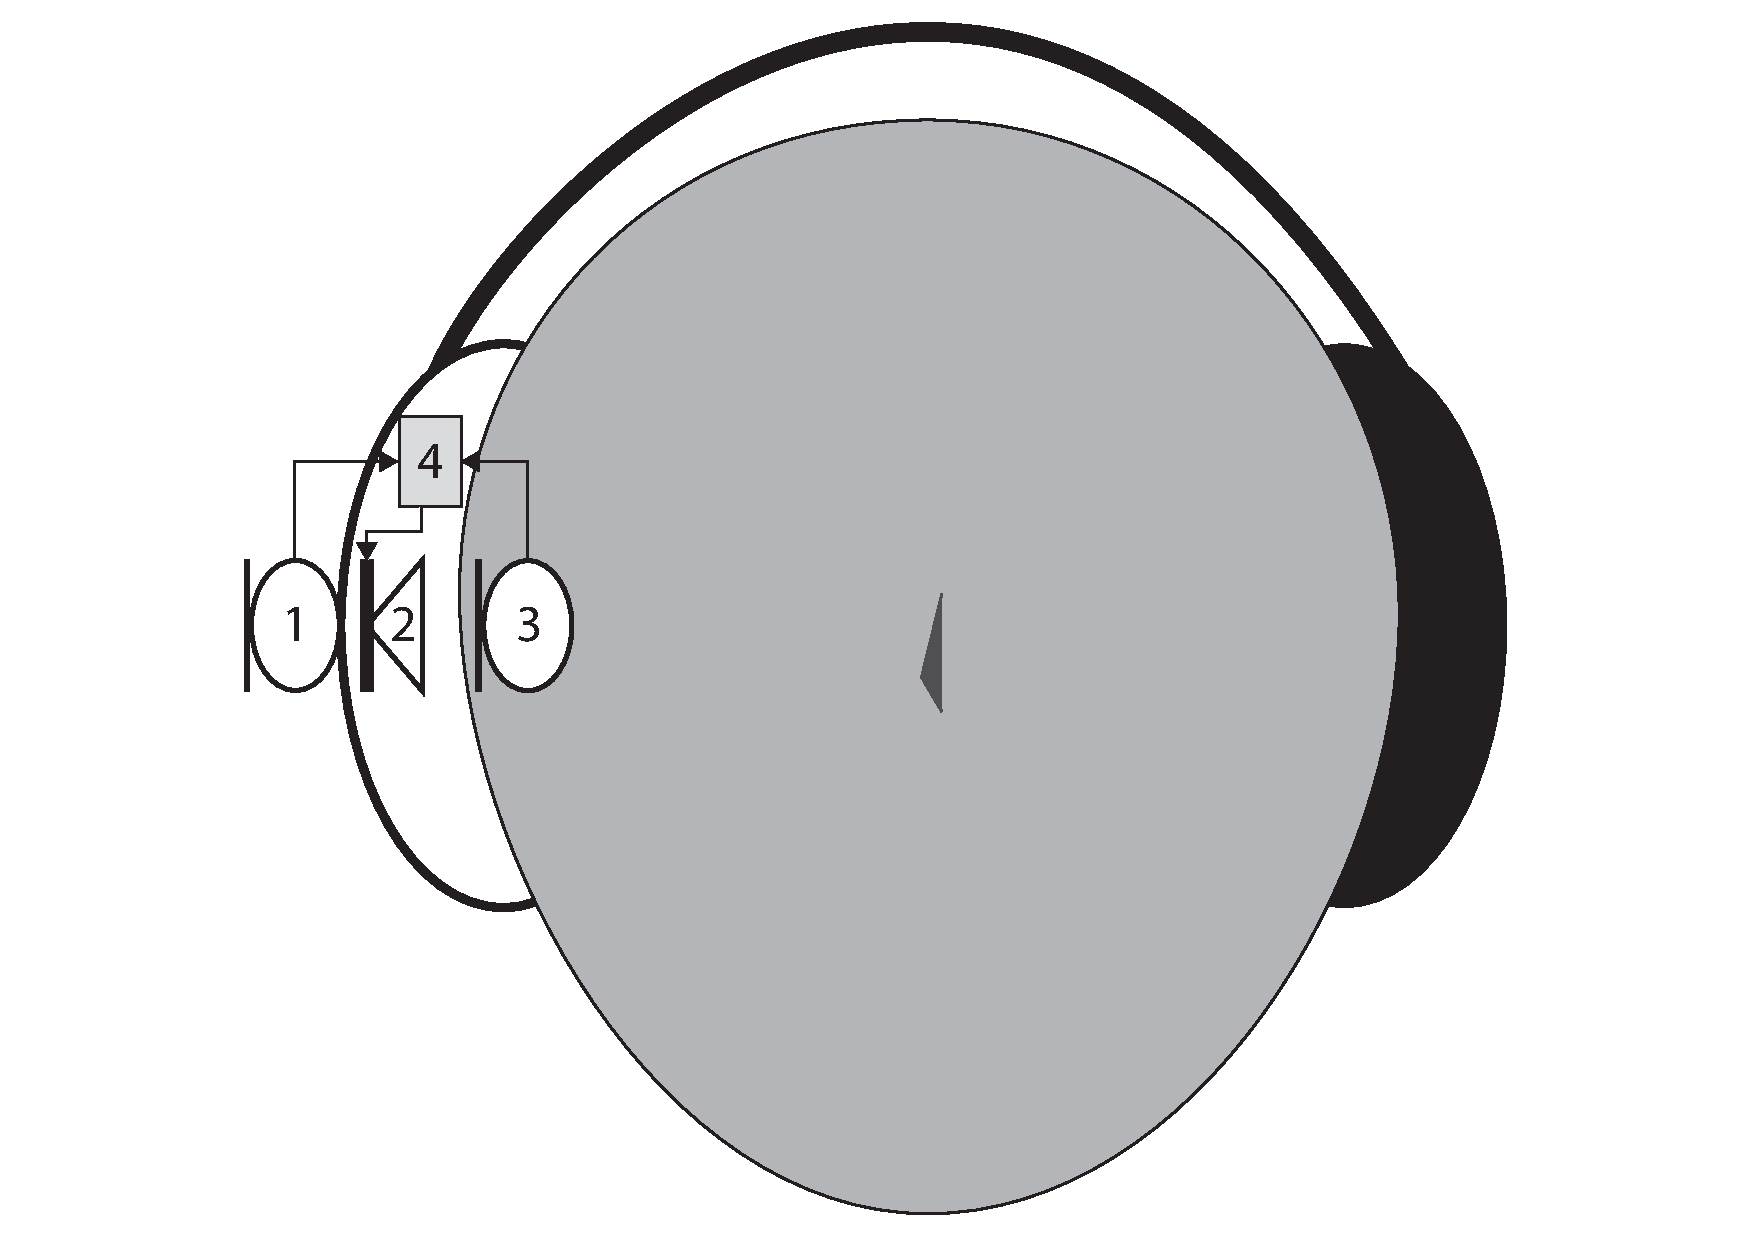
\includegraphics[width=1\columnwidth]{figures/ArticleIllustrations/SystemOverview}
%	\caption{System Overview}
%	\label{fig:SystemOverview}
%\end{figure}



\subsection{Feedforward ANC using FXLMS}
%The adaptive feedforward ANC system is shown on \autoref{fig:ANCFeedforward}


The system in \autoref{fig:ANCFeedforward} outputs a control signal $y[n]$, which ideally is a counter-phase signal of the noise. The signal is generated by inputting the reference signal $x[n]$ into a control filter consisting of adaptive coefficients $b[z]$ representing the transfer function from the reference microphone to the headphone loudspeaker. The coefficients are adapted using the FXLMS algorithm. The FXLMS algorithm inputs the filtered reference $f[n]$ signal along with the error signal $e[n]$. The filtered reference signal is used combined with the error signal to determine new optimal coefficients for the control filter, this is shown in equation \ref{eq:FXLMS}. The signals from (1)(3) are converted to the digital domain using an ADC and anti aliasing filters (AA) before processing. When processed, the output $y[n]$ is reconstructed and converted using a DAC.

 \vspace{-4mm}
{
	%\centering
	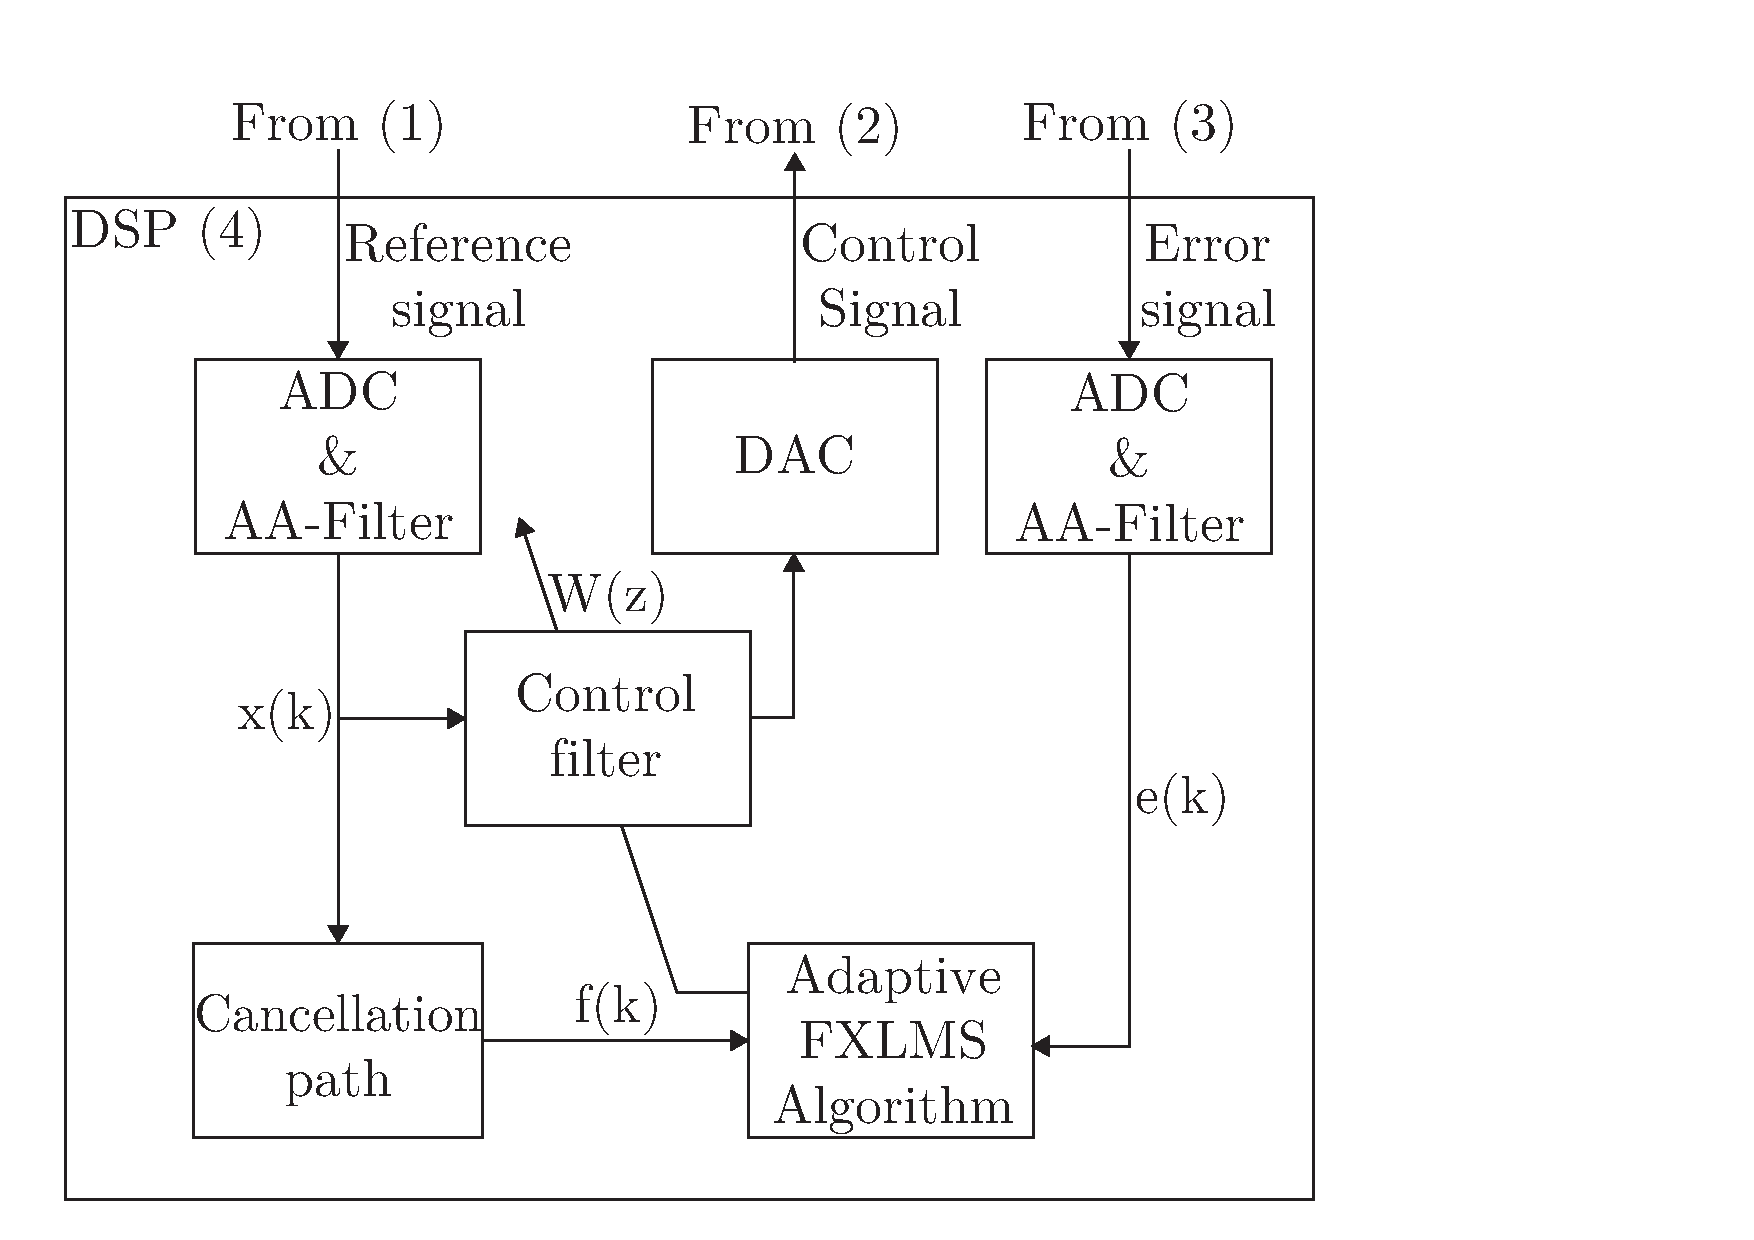
\includegraphics[width=1\columnwidth]{figures/ArticleIllustrations/ANCFeedForward}
	\captionof{figure}{Adaptive feedforward ANC system.}
	\label{fig:ANCFeedforward}
}

%\begin{figure}[H]
%	\centering
%	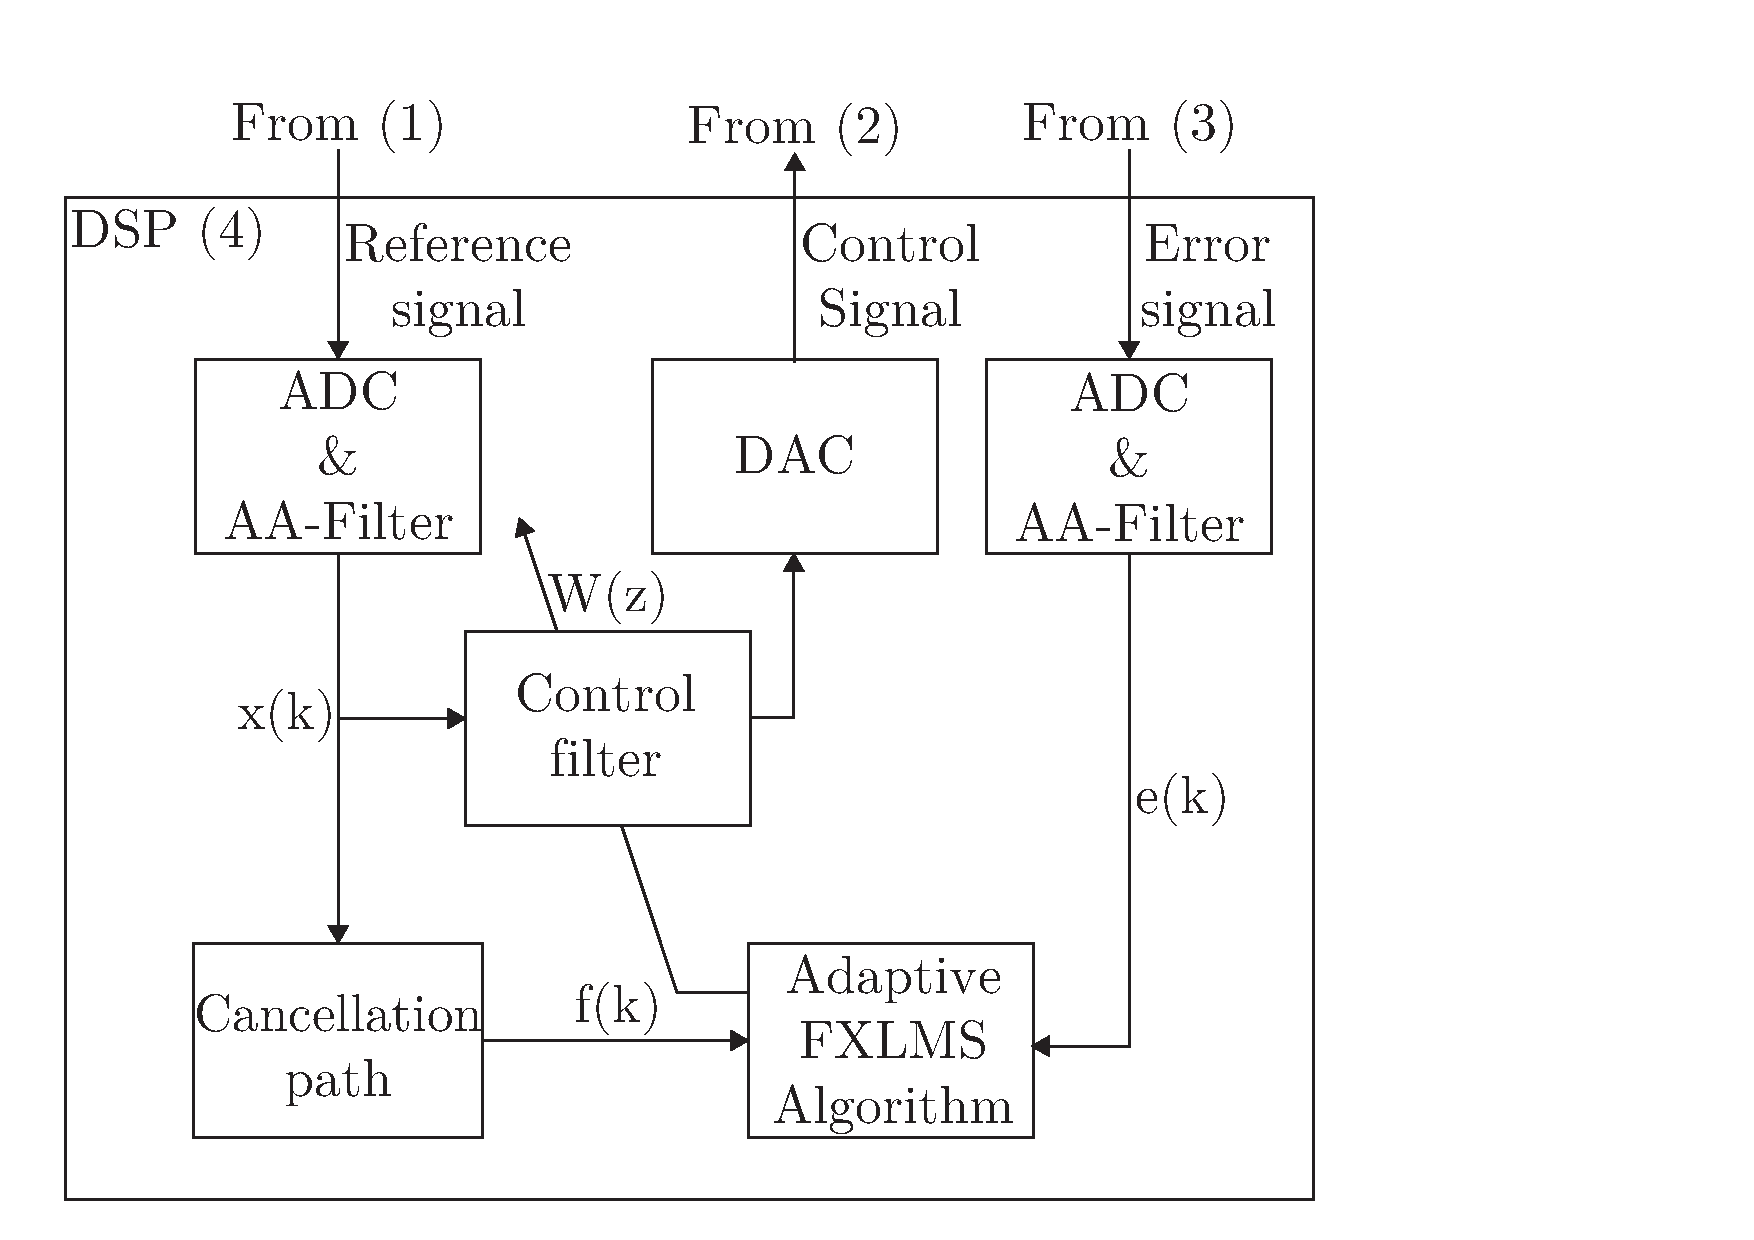
\includegraphics[width=1\columnwidth]{figures/ArticleIllustrations/ANCFeedForward}
%	\caption{Adaptive feedforward ANC system}
%	\label{fig:ANCFeedforward}
%\end{figure}


\textbf{Control Filter} The filter, shown in equation \ref{eq:Output}, is initialized with the inverse of the measured impulse response of the represented transfer function. An order of 256 taps is chosen based on subjective testing in simulation.
\vspace{-3mm} % yeah I know - Sorry Mikkel!
\begin{equation}\label{eq:Output}
y[n]=\sum_{j=0}^{L-1}b_j[n]x[n-j]
\end{equation}
where $b_j[n]$ is the weight coefficients written as  $b[n]=[b_0[n],b_1[n], \cdots, b_{L-1}[n]]^T$.

\textbf{FXLMS} is the optimization algorithm which updates the control filter coefficients using the FXLMS method shown in \autoref{eq:FXLMS}.
\begin{equation}\label{eq:FXLMS}
b_j[n+1] = b_j[n] - 2\mu e[n]f[n-j]
\end{equation}
where $\mu$ is the convergence factor, $e[n]$ is the error and $f[n]$ is the reference convolved with the Cancellation Path.

\textbf{Cancellation Path} (CP) is the transfer-function from the headphone loudspeaker to the error microphone. In the literature \cite{Hansen} the CP is adaptively adjusted, but it is assumed constant because the position of the headphone does not change while measured on a Head and Torso Simulator (HATS). This assumption is made because it is irrelevant for verifying if LP is a plausible solution. 


%When implementing the system, delays exist due to the anti-aliasing and reconstruction filters. The delays of the system exceeds the propagation time of sound from the reference microphone to the headphone loudspeaker resulting in poor performance. Therefore an LP-algorithm is proposed to predict future samples in order to decrease the effect of the time delays.

\subsection{Characteristics of Speech}
Speech can be split into two main classes, voiced and unvoiced. Voiced sounds are characterized by a strong periodicity, with the fundamental frequency referred to as the pitch frequency (50 - 500 Hz). Unvoiced sounds are characterized as random. Speech is a non stationary signal and can only be assumed Wide Sense Stationary (WSS) for periods of 20 - 30 ms \cite{Speech}. 

\subsection{Linear Prediction of Speech}
In order to predict future samples the Auto Correlation Function (ACF), used in LP, of speech must be estimated in frames. The outlines of the prediction system is shown in figure \ref{fig:LinearPredictionOverview}.

\begin{figure}[H]
	\centering
	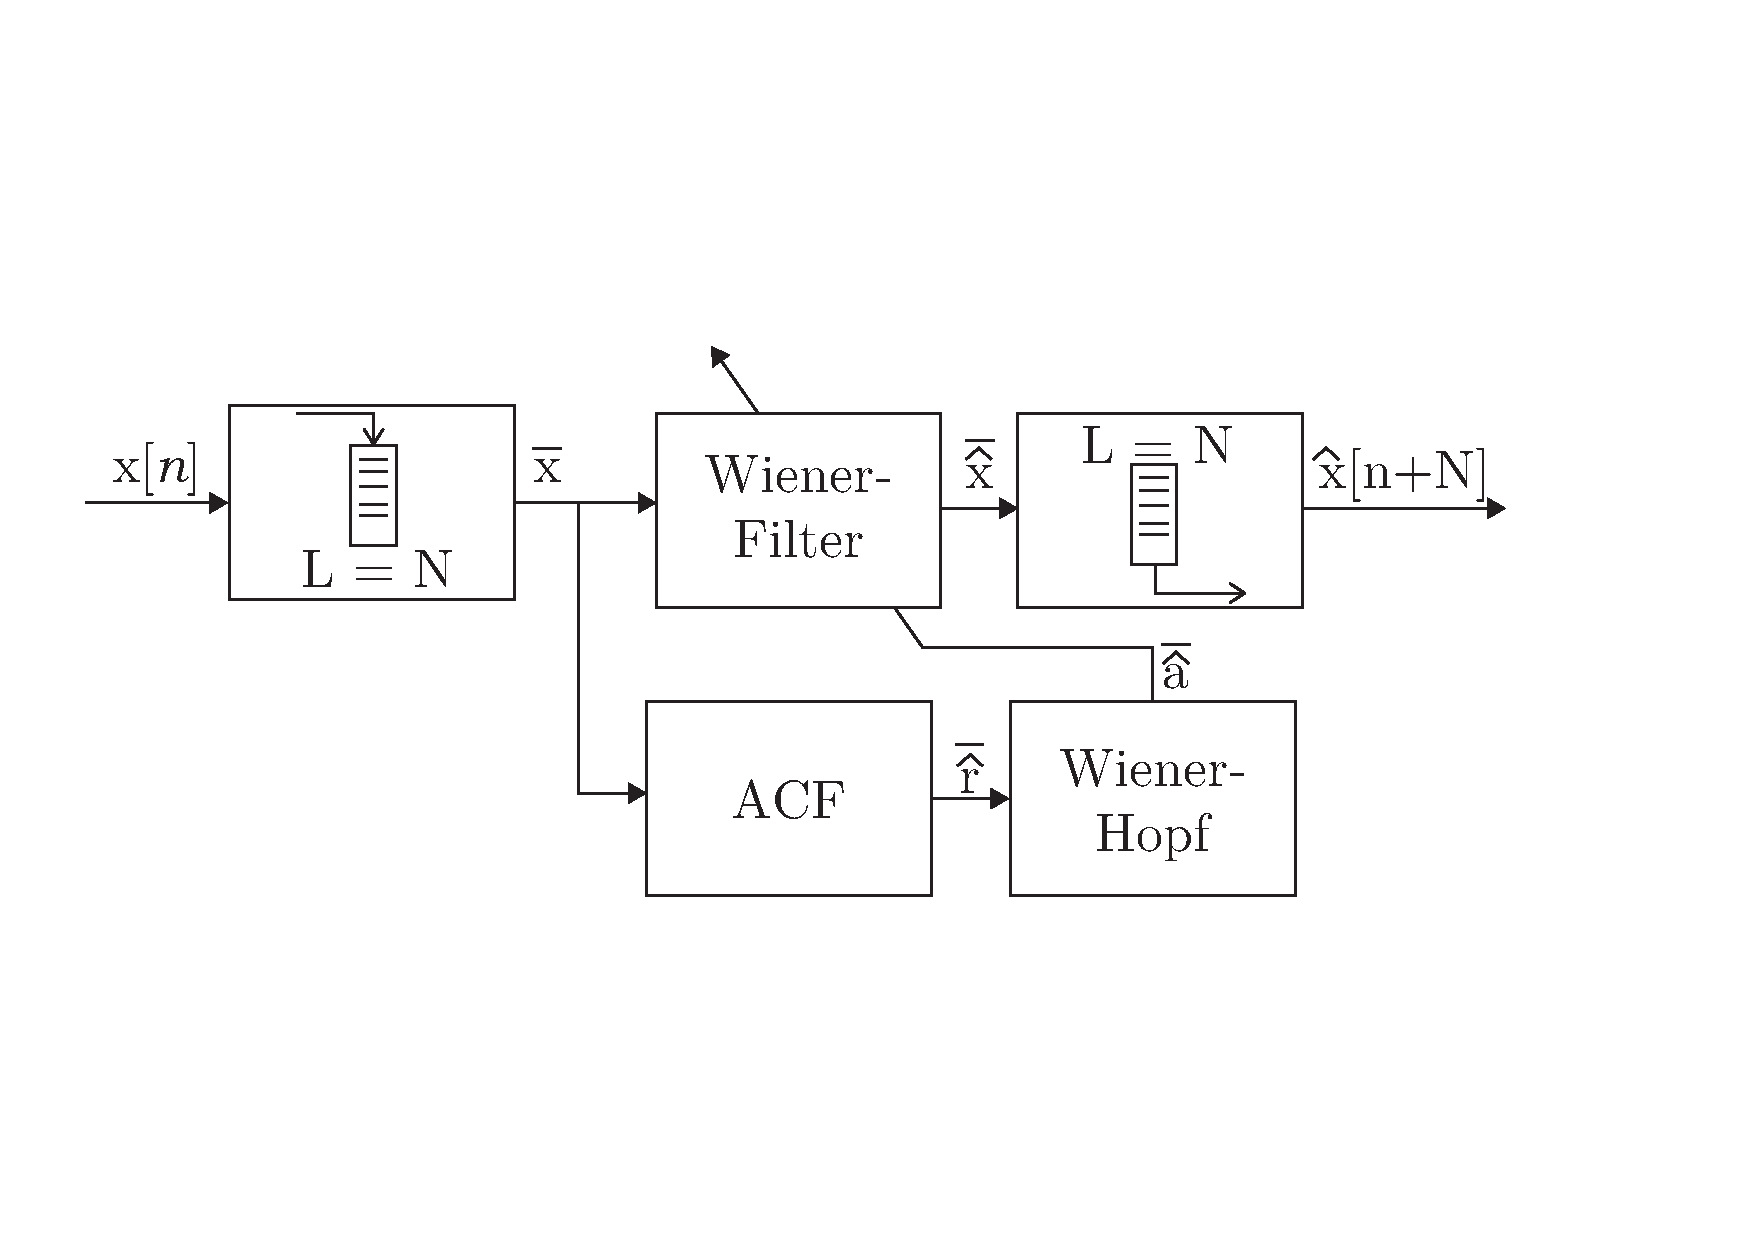
\includegraphics[width=\columnwidth]{ArticleIllustrations/WienerHopf}
	\caption{Linear prediction system.}
	\label{fig:LinearPredictionOverview}
\end{figure}


Utilizing a nonrecursive estimation of the ACF, shown in \autoref{eq:nonrecursive}, it is possible to determine the linear prediction coefficients $\hat{\bar{a}}$ (LPCs) used for predicting future samples \cite{LinearPrediction}. When estimating the ACF of the input ($x$) a Hamming window ($w$) is applied.
\begin{equation}\label{eq:nonrecursive}
%%r_x[l,m] = \sum^{m}_{n=m-N+1+\left| l\right|} x_l[n]w_l[m-n]
\hat{r}_x[l] = \sum^{N}_{n=\left| l\right|} x_l[n]w_l[N-n]
\end{equation}
%\begin{multline}\label{eq:nonrecursive}
%R[l,m] = \sum^{m}_{n=m-N+1+\left| l\right|} \\ x[n]w[m-n] x[n-\left| l\right|]w[m-n+\left| l\right|]
%\end{multline}
%\begin{equation}
%R[l,m]=\sum^{m}_{n=m-N+1+\left| l\right|}x[n]w[m-n] x[n-\left| l\right|]w[m-n+\left| l\right|]
%\end{equation}
where $x_l[n]=x[n]x[n-l]$, $w_l[n]=w[n]w[n+l]$, $l$ is the lag and $N$ is the frame size.

The LPCs are determined using \autoref{eq:normal}, known as the Wiener-Hopf equation.
\begin{equation}\label{eq:normal}
\hat{R}  \bar{a} = -\bar{\hat{r}}_x
\end{equation}
where $\hat{R}$ is the covariance matrix $\hat{C}_{xx}$, $\bar{\hat{a}}$ is the LPCs $\bar{\hat{a}} = [\hat{a}_1 , \hat{a}_2, \cdots, \hat{a}_N]^T$ and $\bar{\hat{r}}_x$ is the ACF, $\bar{\hat{r}}_x = [\hat{r}_x[1] , \hat{r}_x[2], \cdots, \hat{r}_x[N]]^T$.

\autoref{eq:normal} can be rewritten as shown in \autoref{eq:normal2} yielding the LPCs directly.  
 \begin{equation}\label{eq:normal2}
\bar{\hat{a}} = \hat{-R^{-1}} \bar{\hat{r}}_x
\end{equation}
Calculating $\hat{R^{-1}}$ is computationally heavy on a DSP. To estimate the LPCs the Levinson-Durbin method is used \cite{LinearPrediction}. Prediction using Wiener filtering, shown in equation \ref{eq:Predictor}, can then be applied to the current frame for prediction of the next frame. 

\begin{equation}\label{eq:Predictor}
\hat{x}[n+1] =- \sum^{N}_{i=1}\hat{a}_ix[n-i]
\end{equation}

Using equation \ref{eq:Predictor} in cascade where $\hat{x}[n+2]$ is estimated using $\hat{x}[n+1]$ and $x[n]$. The predicted frame is then used as input for the ANC system.

\subsection*{Feedforward LP FXLMS}


%\section*{Results}
\subsection{Prediction Gain}
For the purpose of testing LP prediction gain (PG) shown in \autoref{eq:PG} will be used. 
\begin{equation}\label{eq:PG}
PG = 10 log_{10}\bigg(\frac{\sigma^2_x}{\sigma^2_\varepsilon}\bigg) = 10 log_{10}\bigg(\frac{E\{x^2[n]\}}{E\{\varepsilon^2[n]\}}\bigg)
\end{equation}
where PG is the ratio between the variance of the input signal $x[n]$ and the variance of the prediction error $\varepsilon$ in (dB). The higher the PG the better the prediction is.



\subsection{Determining System Parameters}
The parameters which should be detemined are $fs$, $P$, $N$, $O$, and $M$ using \autoref{eq:PG}.         
The PG of variable $fs$ is shown on \autoref{fig:fsPredict}.

\begin{figure}[H]
	\centering
	\textbf{\textit{Here is going to be a graph of PG determined by fs}}
	\caption{PG }
	\label{fig:fsPredict}
\end{figure}


%These are detemined respectively using a Prediction Gain ($PG$) to find the optimum value. 
The PG of variable $N$, $O$ and $M$ is seen on \autoref{fig:PredictParameters}. 
\begin{figure}[H]
	\centering
	\textbf{\textit{Here is going to be a graph of PG determined by N}}
	\textbf{\textit{Here is going to be a graph of PG determined by O}}
	\textbf{\textit{Here is going to be a graph of PG determined by M}}
	\caption{PG }
	\label{fig:PredictParameters}
\end{figure}

\subsection{Simulation of Feedforward LP FXLMS}

\begin{figure}[H]
	\centering
	\tikzsetnextfilename{DelayRatio}
	% This file was created by matlab2tikz.
%
%The latest updates can be retrieved from
%  http://www.mathworks.com/matlabcentral/fileexchange/22022-matlab2tikz-matlab2tikz
%where you can also make suggestions and rate matlab2tikz.
%
\definecolor{mycolor1}{rgb}{0.00000,0.44700,0.74100}%
\definecolor{mycolor2}{rgb}{0.85000,0.32500,0.09800}%
%
\begin{tikzpicture}

\begin{axis}[%
width=3in,
height=1.75in,
scale only axis,
xmin=0,
xmax=50,
xmajorgrids,
xlabel={Delay [100 $\times$ samples]},
ymin=0,
ymax=70,
ylabel style={yshift=0.3em},
xlabel style={yshift=-0.2em},
ytick={0,10,...,70},
ymajorgrids,
ylabel={Attenuation [dB]},
xticklabel shift={.1cm},
yticklabel shift={.1cm},
axis background/.style={fill=white}
]
\addplot [color=mycolor2,solid,line width=1.5pt,forget plot]
  table[row sep=crcr]{%
2	66.5420250310586\\
4	52.9717264302022\\
6	49.4175149424998\\
8	46.8717703569681\\
10	47.5886347675082\\
12	48.5221420089092\\
14	36.1913078215459\\
16	24.6480360536532\\
18	18.5625963047043\\
20	15.9345988709594\\
22	15.2225924490026\\
24	14.4941735350858\\
26	13.5145912190769\\
28	12.5242379572864\\
30	11.8400523957144\\
32	11.4203165228037\\
34	11.2428861871564\\
36	11.1050592495872\\
38	10.862823901561\\
40	10.6158645117455\\
42	10.3154480278615\\
44	9.97867799972119\\
46	9.61958031033587\\
48	9.31052791122033\\
50	9.08997582022533\\
};
\addplot [color=mycolor1,line width=1.5pt,solid,forget plot]
table[row sep=crcr]{%
	2	25.5751628128288\\
	4	20.0199680852144\\
	6	17.0442763613153\\
	8	15.1060127156582\\
	10	13.7310612019933\\
	12	12.6685774343164\\
	14	11.7903474171974\\
	16	11.0441690144364\\
	18	10.3883064900616\\
	20	9.78797702825996\\
	22	9.23075404560805\\
	24	8.7110676592604\\
	26	8.22176906503967\\
	28	7.77006791263877\\
	30	7.35426684398216\\
	32	6.94907270624338\\
	34	6.5323972441528\\
	36	6.08060777493347\\
	38	5.57101511941803\\
	40	4.99733350616245\\
	42	4.35167702165293\\
	44	3.61433096515684\\
	46	2.757705271237\\
	48	1.74470077738877\\
	50	0.5254168140125\\
};
\end{axis}
\end{tikzpicture}%
	\caption{Attenuation achieved by the system for different system delays.}
	\label{Fig:Reference to noise ratio}
\end{figure}








% At this point in time all results are not yet certain, however we will give an idea of how they are going to turn out.
% As presented in the paper thus far, we know what kind of noise we would like to cancel out and how we want to do it. The following list tells which graph will be used to show the results of the acceptance tests.

% \begin{itemize}
% \item Prediction gain - The difference between the input signal and the estimated signal, measured in dB. Used in the LP part.
% \item A plot comparison of frequency response between: A pure signal, a signal with FXLMS noise attenuation and a signal with LP combined with FXLMS attenuation
% \item An expansion of \autoref{Fig:Reference to noise ratio}: As of now only attenuation is showed, but in the future another graph in the figure will show the attenuation of the FXLMS combined with LP - which should yield better attenuation at larger delays.

% \end{itemize}




%\vspace{5in}
%  \begin{itemize}
  	\item The AAU poster theme v. 1.1.0 has been tested with baposter v. 2.0, and it can be downloaded from my AAU website \cite{jknaau} or my personal website \cite{jknsqrt-1}.
  	\item If you find a bug in the AAU theme (and not in the baposter template), please do not hesitate to contact me. There is a FAQ at the baposter website \cite{baposter}, if you should have any problems with it.
<<<<<<< HEAD
  \end{itemize}
  
  
%\begin{figure}
%  	\floatbox[{\capbeside\thisfloatsetup{capbesideposition={left,top},capbesidewidth=4cm}}]{HammingNOP10}[\FBwidth]
%  	{\caption{A test figure with its caption side by side}\label{fig:test}}
%  	{\includegraphics[width=5cm]{name}}
%\end{figure}
=======
  \end{itemize}
>>>>>>> 386cdecef39d26e2fa621022e6bf7b02f6531c34

%\bibliography{00setup/mybib}
%\end{multicols}
\newpage


\listoftodos
\newpage
\tableofcontents
\section{Introduction}

All files uses for simulation and evaluation for the following experiements can be found on the attached CD, with this path. \path{CD/Appendix [X] - [Appendix\_name]}. If the reader desired to compare their results to ours, they can take a step lower in the directories and locate the folder \path{Verification Results} within the appendix folder. \textbf{The reader should always something something, results something.}
\newpage




%%%%%%%%%%%%%% Litterature and Appendix %%%%%%%%%%%%%%%%%%%%%%
\bookmarksetup{startatroot}% this is it
\addtocontents{toc}{\bigskip}% perhaps as well



 \newpage
 \fancyhead[RO]{\small Appendix \nouppercase\rightmark} %even page - chapter title
 \fancyhead[LE]{\small Appendix \nouppercase\rightmark} %uneven page - section title
\fancyhead[RE,LO]{}

%%%%%%%%%%%%%% Adjusting the titles and fonts (for the appendix) %%%%%%%%%%%%%%%%%%%%%%
\titlespacing{\chapter}{0pt}{0pt}{10pt}
\titlespacing{\section}{0pt}{0pt}{-5pt}
\titlespacing{\subsection}{0pt}{8pt}{5pt}
\titlespacing{\subsubsection}{0pt}{6pt}{10pt}
\titleformat{\section}[hang]{\Large\bfseries}{\thesection\hsp\textcolor{black}{|}\hsp}{0pt}{\Large\bfseries}
\titleformat{\subsection}[hang]{\fontsize{14}{15}\bfseries}{\thesubsection}{10pt}{\fontsize{14}{15}\bfseries}
\titleformat{\subsubsection}[hang]{\bfseries}{\thesubsubsection}{10pt}{\bfseries}

% \renewcommand{\thesection}{\Alph{section}}
 \setcounter{section}{0}
 \addtocontents{toc}{\protect\setcounter{tocdepth}{0}} 
% \part{Appendix}
 \appendix
% \addcontentsline{toc}{chapter}{Appendix}

\section{Speaker Vibration and Frequency Response}\label{app:journal_1}

The purpose of this test is to examine if there is a correlation between the amount of vibration of a speaker and an increased amount of harmonic distortion. The purpose is also to examined if it is possible to detect when the coil hits the backplate. 

\subsection{Setup}

The setup of this experiment are depicted in Figure \ref{figure:SpeakertestSetup}, where the equipment is catalogued in \autoref{tab:UsedEquipment1}, and described as follows:

\begin{itemize}
\item Distortion and \gls{SPL} will be measured by a microphone at a distance of 1 meter in accordance with IEC 60268-5 Sound System Equipment - Part 5: Loudspeaker
\item Vibration will be measured by a Brüel \& Kjear Type 4344 accelerometer, placed at:
\begin{itemize}
\item The backplate of the lowest woofer
\item High, inside and on the back of the enclosure 
\end{itemize}
\item The speaker will be driven by a Crown Studio Reference I amplifier.
\item The ADC/DAC will convert measurements from accelerometers and microphone and relay to a computer via SPDIF.
\begin{itemize}
\item Both accelerometer and microphone is calibrated into outputting -37 dB at respectively 1 G and 94 dB \gls{SPL}.
\item All recordings are synchronised and timestamped with by looping the test file back into the converter.
\end{itemize}
\item The computer will be logging data with a RME HammerFall DIGI 96-PDST sound card and Adobe Audition.
\end{itemize}

Furthermore the speaker will be placed in the anechoic room to eliminate any external disturbances corresponding to the requirements demanded in the 
IEC 60268-5 standard.

\subsection*{Test Setup}

\subsection*{Equipment used and AAU-no.}

\begin{table}[H]
\centering
\ra{1.3}
\begin{tabular}{S[table-format=1]ccc} \toprule
    {Item} & {Description} & {AAU-no} \\ \bottomrule 
    1      &  B \& K Accelerometer Type 4319  & 06598   \\ 
    2      &  B \& K Accelerometer Type 4333  & 06596   \\ 
    3      &  B \& K 2-channel Accelerometer Pre-amp Type 2622  & 07013   \\
    4      &  B \& K Microphone Type 4165  & 08132   \\
    5      &  Gras - 26AK Pre-amp & 52665   \\
    6      &  B \& K Microphone Power supply Type 2804  & 07304   \\
    7      &  Crown Studio Reference I Amplifier & 52614   \\
    8      &  BEHRINGER digital A/D \& D/A Converter - Model ADA8000   & 56545   \\
    9      &  B \& K Accelerometer calibrator 4294 & 08023   \\
    10     &  B \& K Microphone calibrator 4231 & 78301   \\
    11     &  RME HammerFall DIGI 96-PDST sound card & 60919  \\
    11     &  Passive Dali Zensor 5 AX & NaN  \\ \bottomrule 
\end{tabular}
\caption{Table over equipment used in the test}
\label{tab:UsedEquipment1}
\end{table}
\vspace{-5mm}


\subsection{Procedure}\label{sec:SpeakerTestProcedure1}

The producer for this experiment is described as follows:
\vspace{-5mm}
\begin{enumerate}
\item Adjust volume on the amplifier to +3 dB gain.
\item Vacate the anechoic room and seal the room.
\item Start recording in Adobe Audition for:
\begin{itemize}
\item Driver and enclosure accelerometer
\item Microphone and playback loop
\end{itemize}
\item Playback file \path{chirp.wav}, which is a sinusoidal sweep from 2.4 kHz to 10 Hz. The duration of the sweep is 30 seconds and the sweep is linear. The amplitude is 0 dBFS.
\item After playback, stop recording all channels
\item Save recordings as \path{.wav} file
\item Enter room and adjust amplifier by +1 dB
\item Repeat step 2 through 7 until the speaker breaks.
\end{enumerate}

The \path{chirp.wav} are located at:\\
\scalebox{0.7}{
\path{CD://Maalinger/Maalinger030316 - Loudspeaker test/Measurements030316/chirp.wav}}\\




\subsection{Data Extraction}


It was possible to increase the volume by 19 dB until the loudspeaker unit got to damaged. The gain was linear increased by 1 dB, starting at 3 dB, until the 20th test were the loudspeaker unit failed. This results in 20 usable data sets.

The recordings can be found on:\\
\scalebox{0.7}{
\path{CD://Maalinger/Maalinger030316 - Loudspeaker test/Measurements030316/}}
And is indexed in folders \scalebox{0.8}{\path{Measure_X}}, where X corresponds to the test number. Every measurements inside is denoted as:
\begin{itemize}
\item Accelerometer on driver: \scalebox{0.8}{\path{Acc driver_0XX}}
\item Accelerometer in enclosure: \scalebox{0.8}{\path{Acc enclosure_0XX}}
\item Microphone: \scalebox{0.8}{\path{Mic_0XX}}
\item Playback loop: \scalebox{0.8}{\path{Reference_0XX}}
\end{itemize}

The Script used to create all graphs are located at:\\
\scalebox{0.7}{
\path{CD://Maalinger/Maalinger030316 - Loudspeaker test/Measurements030316/MeasurementAnalysis.m}}\\
Figures used in the following \ref{subsec:Raw_data_1} and Dataset 1 though 20 can be found compiled in a combined file at:
\scalebox{0.7}{
\path{CD://Maalinger/Maalinger030316 - Loudspeaker test/Measurements030316/AlleSamlet.pdf}}


\subsubsection{Raw Data}\label{subsec:Raw_data_1}

For each of the test four measurements was taken. These are the accelerometer placed on the driver and enclosure, the microphone and a reference to synchronize the measurements. 

As previously stated there are in total 20 datasets each containing four measurements, namely the vibrations from the enclosure and driver, the sound pressure from the microphone, and lastly a reference signal to synchronize all data. The amount of data is therefore large and only relevant datasets will be presented. The first dataset from the test is shown in \autoref{fig:raw1}.


%\begin{figure}[H]
%\centering
%\begin{subfigure}[t]{0.335\textwidth}
%	\tikzsetnextfilename{Raw_Driver1}
%	\input{figures/Forsog1/Driver1.tex}
%	\caption{Vibration from driver.}
%	\label{fig:raw_driver1}
%\end{subfigure}
%\begin{subfigure}[t]{0.3\textwidth}
%	\tikzsetnextfilename{Raw_Enclosure1}
%	\input{figures/Forsog1/Enclosure1.tex}
%	\caption{Vibration from enclosure.}
%	\label{fig:raw_enclosure1}
%\end{subfigure}
%\begin{subfigure}[t]{0.3\textwidth}
%	\tikzsetnextfilename{Raw_microphone1}
%	\input{figures/Forsog1/Microphone1.tex}
%	\caption{Sound pressure from microphone.}
%	\label{fig:raw_microphone1}
%\end{subfigure}
%\caption{The measured data of (a) the vibration on the driver, (b) the vibration on the enclosure, and (c) the sound pressure from the microphone. Dataset 1.}
%\label{fig:raw1}
%\end{figure} 


Looking at the first dataset reveals that there are mechanical issues with the loudspeaker. In \autoref{fig:raw_driver1} there is a strong indication of a resonance frequency at 25 seconds with a peak amplitude on approximately 0.02. A similar observation can be found in \autoref{fig:raw_enclosure1} which shows the vibration measured by the accelerometer placed on the enclosure where a resonance frequency appears after 25 seconds. Another mechanical resonance frequency can be found located after 14 seconds for the enclosure. The sound pressure level measured by the microphone is in contrast fairly linear compared to the measured vibrations. Dataset 10 is shown in \autoref{fig:raw10} where the gain is increased by 10 dB.

%\begin{figure}[H]
%\centering
%\begin{subfigure}[t]{0.335\textwidth}
%	\tikzsetnextfilename{Raw_Driver10}
%	\input{figures/Forsog1/Driver10.tex}
%	\caption{Vibration from driver.}
%	\label{fig:raw_driver10}
%\end{subfigure}
%\begin{subfigure}[t]{0.3\textwidth}
%	\tikzsetnextfilename{Raw_Enclosure10}
%	\input{figures/Forsog1/Enclosure10.tex}
%	\caption{Vibration from enclosure.}
%	\label{fig:raw_enclosure10}
%\end{subfigure}
%\begin{subfigure}[t]{0.3\textwidth}
%	\tikzsetnextfilename{Raw_microphone10}
%	\input{figures/Forsog1/Microphone10.tex}
%	\caption{Sound pressure from microphone.}
%	\label{fig:raw_microphone10}
%\end{subfigure}
%\caption{The measured data of (a) the vibration on the driver, (b) the vibration on the enclosure, and (c) the sound pressure from the microphone. Dataset 10.}
%\label{fig:raw10}
%\end{figure} 

The measurements from dataset 10 is very similar to the measurements seen in dataset 1. Since no particular change is happening between dataset 1 to 10 it is assumed that the performance of the loudspeaker remains good. A further analysis of the performance speaker will be done in the analysis of the harmonic distortion section to examine the amount of harmonic distortion present. Dataset 14 is shown in \autoref{fig:raw14}. 

%\begin{figure}[H]
%\centering
%\begin{subfigure}[t]{0.335\textwidth}
%	\tikzsetnextfilename{Raw_Driver14}
%	\input{figures/Forsog1/Driver14.tex}
%	\caption{Vibration from driver.}
%	\label{fig:raw_driver14}
%\end{subfigure}
%\begin{subfigure}[t]{0.3\textwidth}
%	\tikzsetnextfilename{Raw_Enclosure14}
%	\input{figures/Forsog1/Enclosure14.tex}
%	\caption{Vibration from enclosure.}
%	\label{fig:raw_enclosure14}
%\end{subfigure}
%\begin{subfigure}[t]{0.3\textwidth}
%	\tikzsetnextfilename{Raw_microphone14}
%	\input{figures/Forsog1/Microphone14.tex}
%	\caption{Sound pressure from microphone.}
%	\label{fig:raw_microphone14}
%\end{subfigure}
%\caption{The measured data of (a) the vibration on the driver, (b) the vibration on the enclosure, and (c) the sound pressure from the microphone. Dataset 14.}
%\label{fig:raw14}
%\end{figure} 

While most of the measurements show the exact same characteristics as previous datasets, a slight change occurs in the end of the vibration measured on the driver in \autoref{fig:raw_driver14} and the sound pressure level in \autoref{fig:raw_microphone14}. After approximately 29 seconds a peak is observed in \autoref{fig:raw_driver14} which could indicate that the coil at that point hit the back plate of the driver. A further examination will be made in a later section. The measurements from the microphone, also show that a peak occurs at the same point, which most likely will cause the amount of harmonic distortion to increase. Dataset 19, which is the last dataset before the loudspeaker break down, is shown in \autoref{fig:raw19}.

%\begin{figure}[H]
%\centering
%\begin{subfigure}[t]{0.335\textwidth}
%	\tikzsetnextfilename{Raw_Driver19}
%	\input{figures/Forsog1/Driver19.tex}
%	\caption{Vibration from driver.}
%	\label{fig:raw_driver19}
%\end{subfigure}
%\begin{subfigure}[t]{0.3\textwidth}
%	\tikzsetnextfilename{Raw_Enclosure19}
%	\input{figures/Forsog1/Enclosure19.tex}
%	\caption{Vibration from enclosure.}
%	\label{fig:raw_enclosure19}
%\end{subfigure}
%\begin{subfigure}[t]{0.3\textwidth}
%	\tikzsetnextfilename{Raw_microphone19}
%	\input{figures/Forsog1/Microphone19.tex}
%	\caption{Sound pressure from microphone.}
%	\label{fig:raw_microphone19}
%\end{subfigure}
%\caption{The measured data of (a) the vibration on the driver, (b) the vibration on the enclosure, and (c) the sound pressure from the microphone. Dataset 19.}
%\label{fig:raw19}
%\end{figure} 

Dataset 19 has the same characteristics as dataset 14, though with a more noticeable peak at 29 seconds for both the measurements from the driver and the microphone. In the last dataset shown in \autoref{fig:raw20}, the loudspeaker breaks down.


%\begin{figure}[H]
%\centering
%\begin{subfigure}[t]{0.335\textwidth}
%	\tikzsetnextfilename{Raw_Driver20}
%	\input{figures/Forsog1/Driver20.tex}
%	\caption{Vibration from driver.}
%	\label{fig:raw_driver20}
%\end{subfigure}
%\begin{subfigure}[t]{0.3\textwidth}
%	\tikzsetnextfilename{Raw_Enclosure20}
%	\input{figures/Forsog1/Enclosure20.tex}
%	\caption{Vibration from enclosure.}
%	\label{fig:raw_enclosure20}
%\end{subfigure}
%\begin{subfigure}[t]{0.3\textwidth}
%	\tikzsetnextfilename{Raw_microphone20}
%	\input{figures/Forsog1/Microphone20.tex}
%	\caption{Sound pressure from microphone.}
%	\label{fig:raw_microphone20}
%\end{subfigure}
%\caption{The measured data of (a) the vibration on the driver, (b) the vibration on the enclosure, and (c) the sound pressure from the microphone. Dataset 20.}
%\label{fig:raw20}
%\end{figure} 

As seen in \autoref{fig:raw_driver20} the loudspeaker unit breaks down at the mechanical resonance frequency for the driver. The reason to why vibrations on the enclosure and sound pressure are still presentthe  after 25 seconds is because the other loudspeaker unit did not entirely break down. Since the loudspeaker unit broke down at the mechanical driver resonance frequency, it would be relevant to examine if there is any correlation as such.



\subsection{Analysis}

\subsubsection{Frequency response}

To determine the frequency response of the vibration from the driver, enclosure and the speaker frequency response a Fast Fourier Transformation (FFT) is applied to all three measurements.

%\begin{figure}[H]
%\centering
%\begin{subfigure}[t]{0.37\textwidth}
%	\tikzsetnextfilename{FFT_driver1}
%	\input{figures/FFT_driver1.tex}
%	\caption{Driver.}
%	\label{fig:FFT_driver1}
%\end{subfigure}
%\begin{subfigure}[t]{0.28\textwidth}
%	\tikzsetnextfilename{FFT_enclosure1}
%	\input{figures/FFT_enclosure1.tex}
%	\caption{Enclosure.}
%	\label{fig:FFT_enclosure1}
%\end{subfigure}
%\begin{subfigure}[t]{0.32\textwidth}
%	\tikzsetnextfilename{FFT_mic1}
%	\input{figures/FFT_mic1.tex}
%	\caption{Microphone.}
%	\label{fig:FFT_mic1}
%\end{subfigure}
%\caption{Frequency response of (a) the vibration on the driver, (b) the vibration on the enclosure, and (c) the speaker. Test 1.}
%\label{fig:FFT1}
%\end{figure}

From \autoref{fig:FFT_driver1} it is seen that the driver has a resonance frequency located at approximately 390 Hz and a dip at 1290 Hz. The enclosure also has a peak located at 390 Hz, but also has another peak located at 1290 Hz which is the opposite to the frequency response of the driver. The speaker frequency response measured by the microphone, shows that the response is flat compared to the two other responses from 10 Hz to 2.4 kHz.

%\begin{figure}[H]
%\centering
%\begin{subfigure}[t]{0.37\textwidth}
%	\tikzsetnextfilename{FFT_driver10}
%	\input{figures/FFT_driver10.tex}
%	\caption{Driver.}
%	\label{fig:FFT_driver10}
%\end{subfigure}
%\begin{subfigure}[t]{0.28\textwidth}
%	\tikzsetnextfilename{FFT_enclosure10}
%	\input{figures/FFT_enclosure10.tex}
%	\caption{Enclosure.}
%	\label{fig:FFT_enclosure10}
%\end{subfigure}
%\begin{subfigure}[t]{0.32\textwidth}
%	\tikzsetnextfilename{FFT_mic10}
%	\input{figures/FFT_mic10.tex}
%	\caption{Microphone.}
%	\label{fig:FFT_mic10}
%\end{subfigure}
%\caption{Frequency response of (a) the vibration on the driver, (b) the vibration on the enclosure, and (c) the speaker. Test 10.}
%\label{fig:FFT10}
%\end{figure}

The frequency response for all three measurements in test 10 is very similar to the frequency response found in test 1. The same applies to all the test from 1 to 10. No noticeable difference between the test is observed.

%\begin{figure}[H]
%\centering
%\begin{subfigure}[t]{0.37\textwidth}
%	\tikzsetnextfilename{FFT_driver19}
%	\input{figures/FFT_driver19.tex}
%	\caption{Driver.}
%	\label{fig:FFT_driver19}
%\end{subfigure}
%\begin{subfigure}[t]{0.28\textwidth}
%	\tikzsetnextfilename{FFT_enclosure19}
%	\input{figures/FFT_enclosure19.tex}
%	\caption{Enclosure.}
%	\label{fig:FFT_enclosure19}
%\end{subfigure}
%\begin{subfigure}[t]{0.32\textwidth}
%	\tikzsetnextfilename{FFT_mic19}
%	\input{figures/FFT_mic19.tex}
%	\caption{Microphone.}
%	\label{fig:FFT_mic19}
%\end{subfigure}
%\caption{Frequency response of (a) the vibration on the driver, (b) the vibration on the enclosure, and (c) the speaker. Test 10.}
%\label{fig:FFT19}
%\end{figure} 

The frequency responses test 19, which is the test before the loudspeaker got damaged, shows little signs of any changes in the frequency responses from the previous tests, thus is not possible to determine if the loudspeaker is close the being damaged alone from the frequency responses.


\subsubsection{Harmonic distortion}

In this section the amount of harmonic distortion of the loudspeaker is analysed, to examine if it is possible to determine the performance of the loudspeaker from harmonics. To analyse the harmonic distortion a spectrogram is used. The spectrogram is a three dimensional plot which shows the frequency, time and magnitude. Basically the spectrogram is an array of multiple FFT each calculated at a given time with a given window.

The advantages of using a spectrogram is that it gives a good overview of the spectral content in the signal at any given time. Since the harmonic frequencies depends on the fundamental frequency, it is better to use a spectrogram rather than a regular FFT, since the spectrogram will reveal all harmonic distortion for all fundamental frequency from 10 Hz to 2.4 kHz. The spectrograms for microphone in dataset 1 and 19 are shown in \autoref{fig:spec_mic}.

%\begin{figure}[H]
%\centering
%\begin{subfigure}[t]{0.47\textwidth}
%	\tikzsetnextfilename{Microphone_spec1}
%	\input{figures/Forsog1/Microphone_spec1.tex}
%	\caption{Microphone dataset 1}
%	\label{fig:spectrogram_mic1}
%\end{subfigure}
%\begin{subfigure}[t]{0.47\textwidth}
%	\tikzsetnextfilename{Microphone_spec19}
%	\input{figures/Forsog1/Microphone_spec19.tex}
%	\caption{Microphone dataset 19}
%	\label{fig:spectrogram_mic19}
%\end{subfigure}
%\caption{The spectrograms of the microphone dataset 1 and 19. The prominent red line is the sine sweep from 2.4 kHz to 10 Hz while the yellow and blue lines along the red line are harmonic distortion.}
%\label{fig:spec_mic}
%\end{figure} 

The spectrograms of dataset 1 and 19 for the microphone, seen in \autoref{fig:spectrogram_mic1} and \autoref{fig:spectrogram_mic1}, show a prominent orange line and three weak blue lines above the red line. It is seen that the orange line is a linear decreasing function from 2.4 kHz to 10 Hz where the frequency is a function of time. This indicates that the red line is the fundamental frequency of the sine sweep from 2.4 kHz to 10 Hz. The yellow line are linear functions of the harmonic distortions. The spectrograms clearly show that increasing the gain will increase the amount of harmonic distortion as well. An interesting observation is the spectral frequency leak that occurs at lower frequencies revealing large amount of distortion at low frequency and high gain. Since the power of the spectrum other than the harmonic frequencies increase, it could indicate that the coil hit the back plate of the driver at this point. From the analysis it can be concluded that the large amount of distortion can indicate that the coil is hitting the back plate of the driver.

The next part will be to analyse if similar observation can be found in the spectrogram for vibration measurements on the driver and the enclosure. 

%\begin{figure}[H]
%\centering
%\begin{subfigure}[t]{0.47\textwidth}
%	\tikzsetnextfilename{Driver_spec1}
%	\input{figures/Forsog1/Driver_spec1.tex}
%	\caption{Driver dataset 1.}
%	\label{fig:spectrogram_driver1}
%\end{subfigure}
%\begin{subfigure}[t]{0.47\textwidth}
%	\tikzsetnextfilename{Driver_spec19}
%	\input{figures/Forsog1/Driver_spec19.tex}
%	\caption{Driver dataset 19.}
%	\label{fig:spectrogram_driver19}
%\end{subfigure}
%\caption{The spectrograms of the driver dataset 1 and 19. The prominent orange line is the sine sweep from 2.4 kHz to 10 Hz while the yellow lines are harmonic distortion.}
%\label{fig:spec_driver}
%\end{figure} 

The spectrograms of dataset 1 and 19 of the driver are seen in \autoref{fig:spec_driver}. From the spectrograms it is seen that the harmonic distortion is also present in the driver measurements as well as the frequency leak at lower frequencies at high gain. Finally the spectrum of the enclosure measurements is examined in \autoref{fig:spec_driver}.

%\begin{figure}[H]
%\centering
%\begin{subfigure}[t]{0.47\textwidth}
%	\tikzsetnextfilename{Enclosure_spec1}
%	\input{figures/Forsog1/Enclosure_spec1.tex}
%	\caption{Enclosure dataset 1.}
%	\label{fig:spectrogram_enclosure1}
%\end{subfigure}
%\begin{subfigure}[t]{0.47\textwidth}
%	\tikzsetnextfilename{Enclosure_spec19}
%	\input{figures/Forsog1/Enclosure_spec19.tex}
%	\caption{Enclosure dataset 19}
%	\label{fig:spectrogram_enclosure19}
%\end{subfigure}
%\caption{The spectrograms of the enclosure dataset 1 and 19. The prominent orange line is the sine sweep from 2.4 kHz to 10 Hz while the yellow lines are harmonic distortion.}
%\label{fig:spec_enclosure}
%\end{figure} 

It is seen that there is considerately more frequency leak throughout the whole spectrum compared to the spectrogram for the driver and microphone. However the measurements from the driver, enclosure, and microphone is the large amount of frequency leak at very low frequencies seen at after 29 seconds.

This section concludes that amount of distortion increases significantly when the gain is increased too. Also, it can be concluded that there is a frequency leak at lower frequencies on both driver, enclosure, and microphone. 



\subsection{Back Plate Hit Detection}\label{sec:hit_detect}

As previously stated, it is possible that the loudspeaker coil hits the back plate of the driver if the coil moves too far back. In the long run this will damage the loudspeaker, and should therefore be avoided. In this section an analysis on how to detect these hits, will be provided. 

The frequency response of a mechanical frame of a loudspeaker has the same characteristics as a low-pass filter. This means, if the coil is hitting the back plate of the driver, it will result in a increase in energy in the low frequency spectrum. As most music and loudspeakers have most of its energy above 50 Hz, it can be assumed that only a back plate hit will generate vibrations at very low frequencies between, for instance, 0 Hz to 20 Hz. To examine if this is true, a section of the dataset 19 of the driver, where a hit is suspected to have occurred, is analysed. The analysed section is seen in \autoref{fig:raw_driver19_windows}.


%\begin{figure}[H]
%\centering
%\begin{subfigure}[t]{0.55\textwidth}
%	\tikzsetnextfilename{raw_driver19_window}
%	\input{figures/raw_driver19_window.tex}
%	\caption{Raw dataset 19 for driver.}
%	\label{fig:raw_driver19_window}
%\end{subfigure}
%%\hspace{6mm} 
%\begin{subfigure}[t]{0.43\textwidth}
%	\tikzsetnextfilename{raw_driver19_window_zoom}
%	\input{figures/raw_driver19_window_zoom.tex}
%	\caption{The grey area zoomed in.}
%	\label{fig:raw_driver19_window_zoom}
%\end{subfigure}
%\caption{The greyed area is analysed to examine if there are any signs of an impulse.}
%\label{fig:raw_driver19_windows}
%\end{figure}

The same window is applied to all datasets for the driver and afterwards spectrum analysed to reveal any increase in low frequent energy. 

%\begin{figure}[H]
%\centering
%\tikzsetnextfilename{FFTFinal}
%\input{figures/Forsog1/FFTFinal.tex}
%\caption{The FFT of the measurements at 80 Hz.}
%\label{fig:FFT_hit}
%\end{figure}

It is seen that the energy for non-harmonic frequencies is increased at very low frequencies as indicated with the arrow. The yellow graph is the first dataset and the red is the tenth dataset. As no hit was observed in the window at dataset 1 and 10, the energy of lower part of the spectrum was not increased. However the suspected hit in dataset 19 has an energy increase in the low frequency spectrum. Note that since the window is 0.25 seconds wide, frequencies below 4 Hz should be discarded.

\subsection{Error sources}

Few errors could have occurred during trials, since the only variable adjusted during between measurements was the gain of the amplifier. There were however problems with moving the setup from the control room were it was calibrated and then moved into the anechoic room. The calibration was done using an visual equalizer where the output was shown with a bar chart hence the data should bee seen with a tolerance of +/- 0.5 dB.

\subsection{Conclusion}
The test concludes that is possible to detect a hit against the back plate. The draw back of using an accelerometer is however that it is not possible to determine a hit before it happens. 



\label{bib:mybiblio}
\bibliography{00setup/mybib}

\end{document}